\documentclass[a4paper, 11pt]{article}
\usepackage{comment} % enables the use of multi-line comments (\ifx \fi) 
\usepackage{pdfpages}
\usepackage{fullpage} % changes the margin

\begin{document}
%Header-Make sure you update this information!!!!
\noindent
\large\textbf{Nick Tyler} \hfill \\
\normalsize Final Project \hfill PHYS 723 \\

\section*{CMS Open Data, $X \rightarrow  \mu \mu$ } 
For my project I used the CMS Open Data platform to get experimental data of proton proton collisions at $7 TeV$ \cite{OpenData}.  I used a set of scripts from GitHub and modified them slightly to read the data and output results for decays to two $\mu$ \cite{GitHub}. For each event the energy and momentum for each $\mu$ was saved as well as the charge of each and the mass of the particle the $\mu$ decayed from. In the end I was able to collect around 3 million individual events.

\section*{$Z^0$ Decays}
To find $Z^0$ decays I first made sure that the decays conserved charge so that $Z^0 \rightarrow  \mu^+ \mu^-$. After the initial charge cut I was left with roughly 2 million neutral decays.  I looked at the mass histogram in the range above $40\,GeV$ to find the $Z^0$ peak around $91\,GeV$.\\
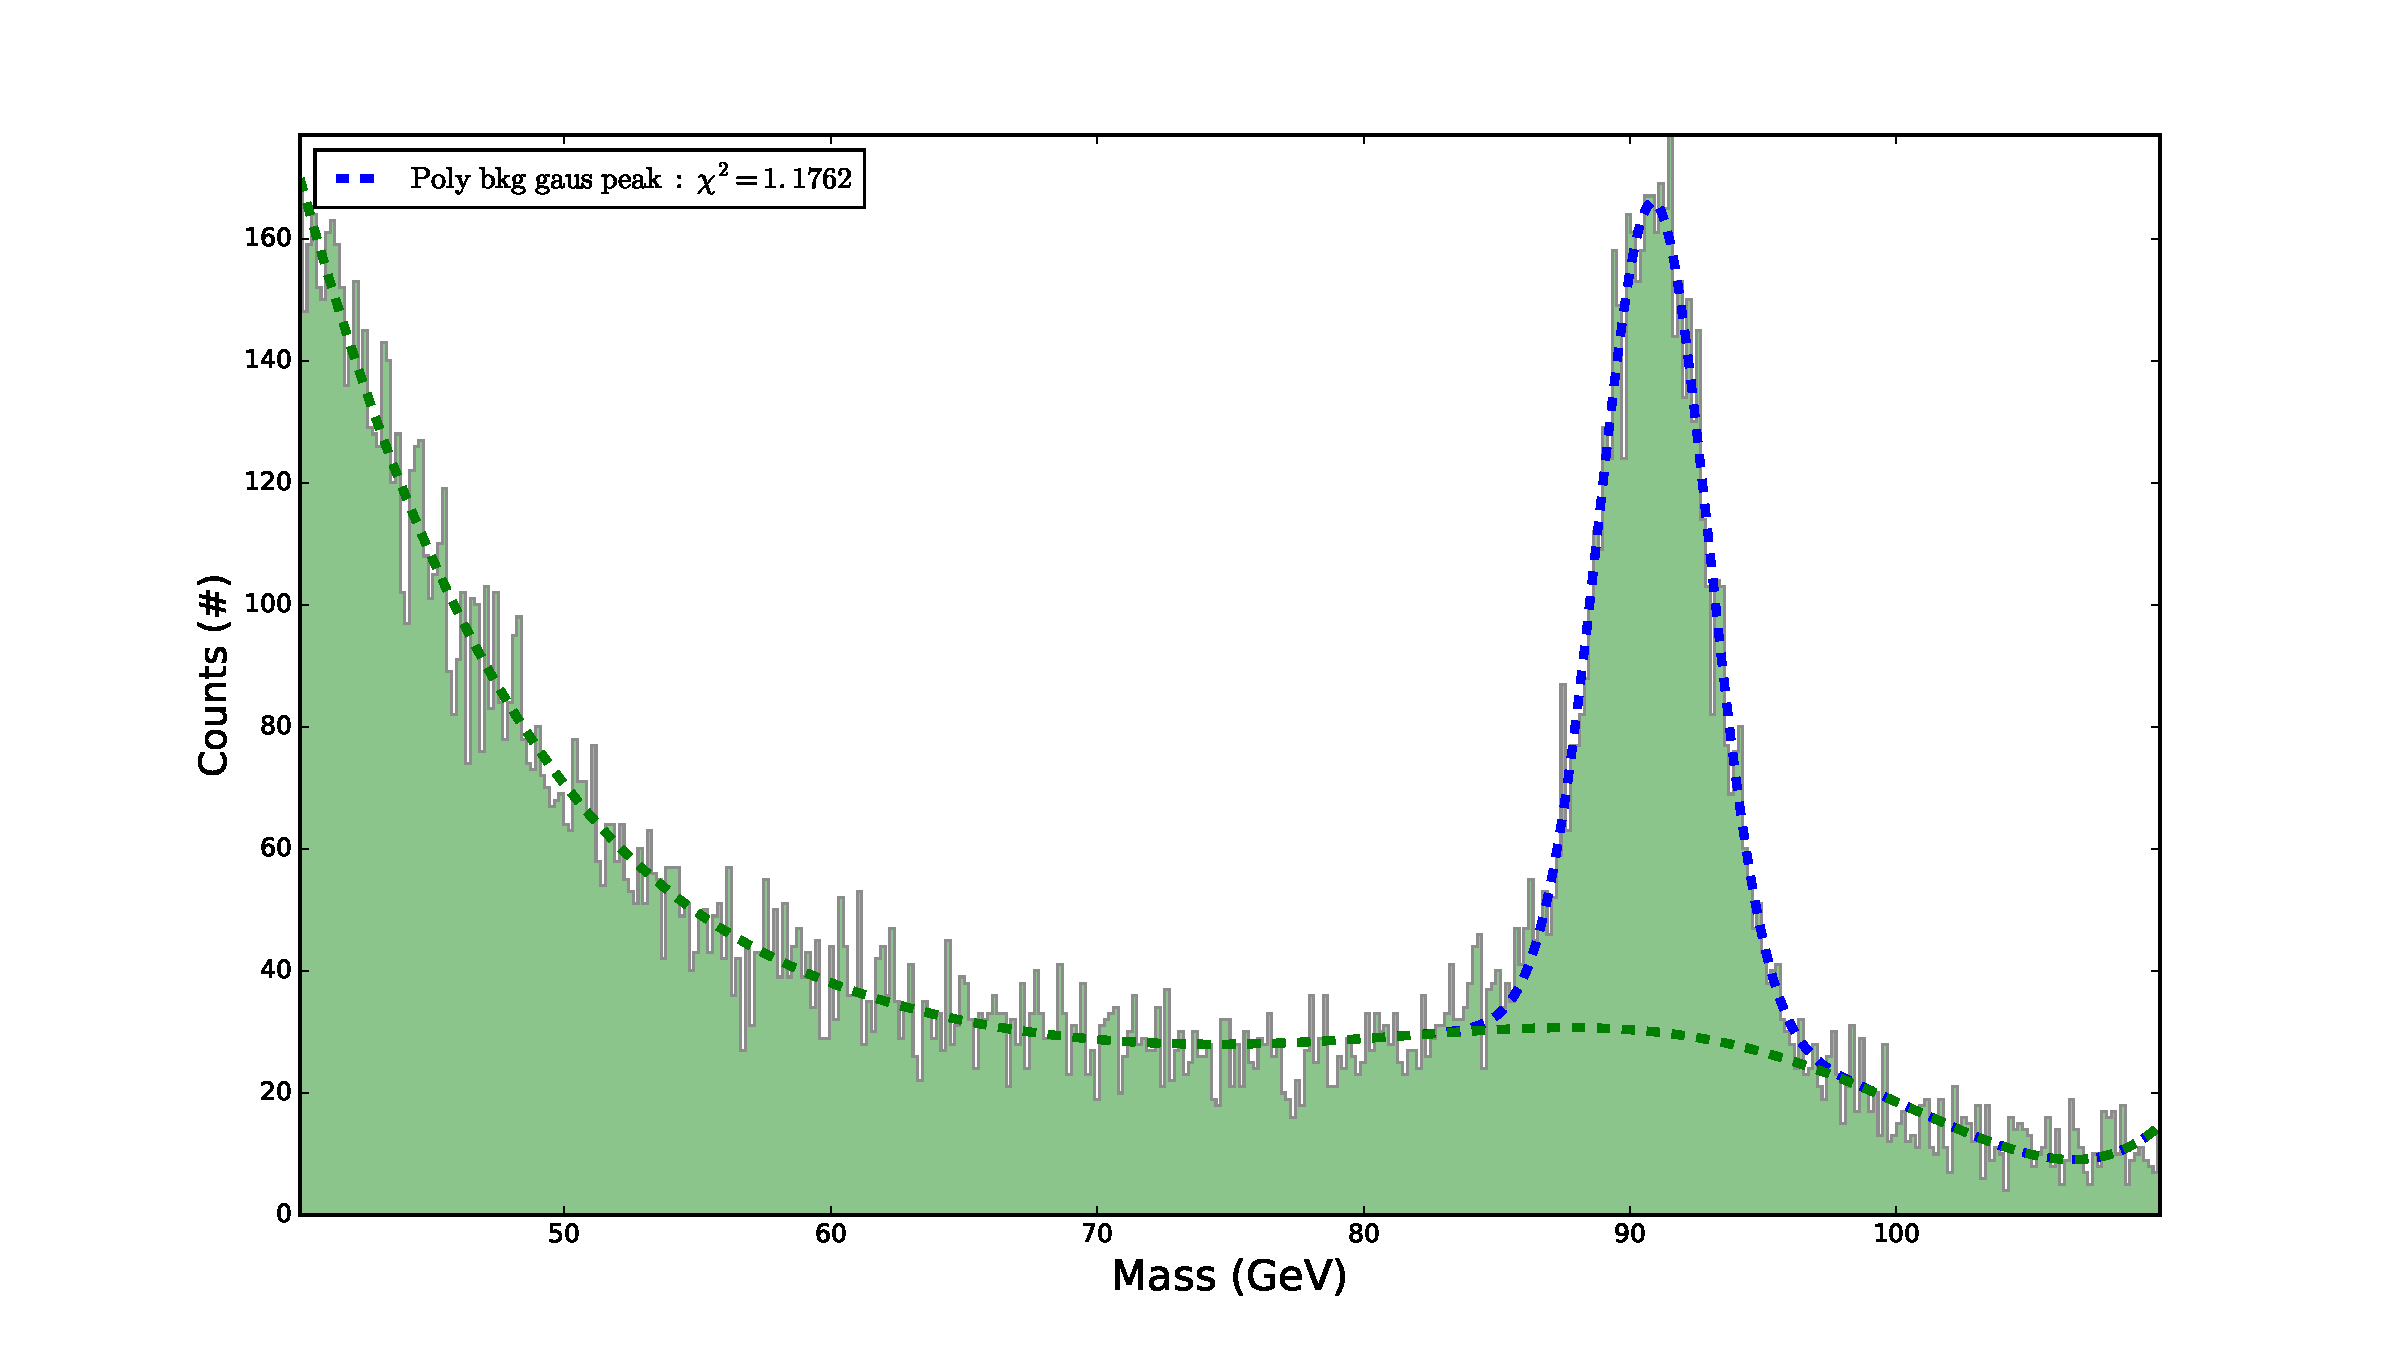
\includegraphics[width=\textwidth]{Z_stuff/Mass_histogram.pdf} \\

I then fit a polynomial background with a Gaussian peak around $91\,GeV$ on the data and used this to subtract away the background to find the $Z^0$ peak. \\

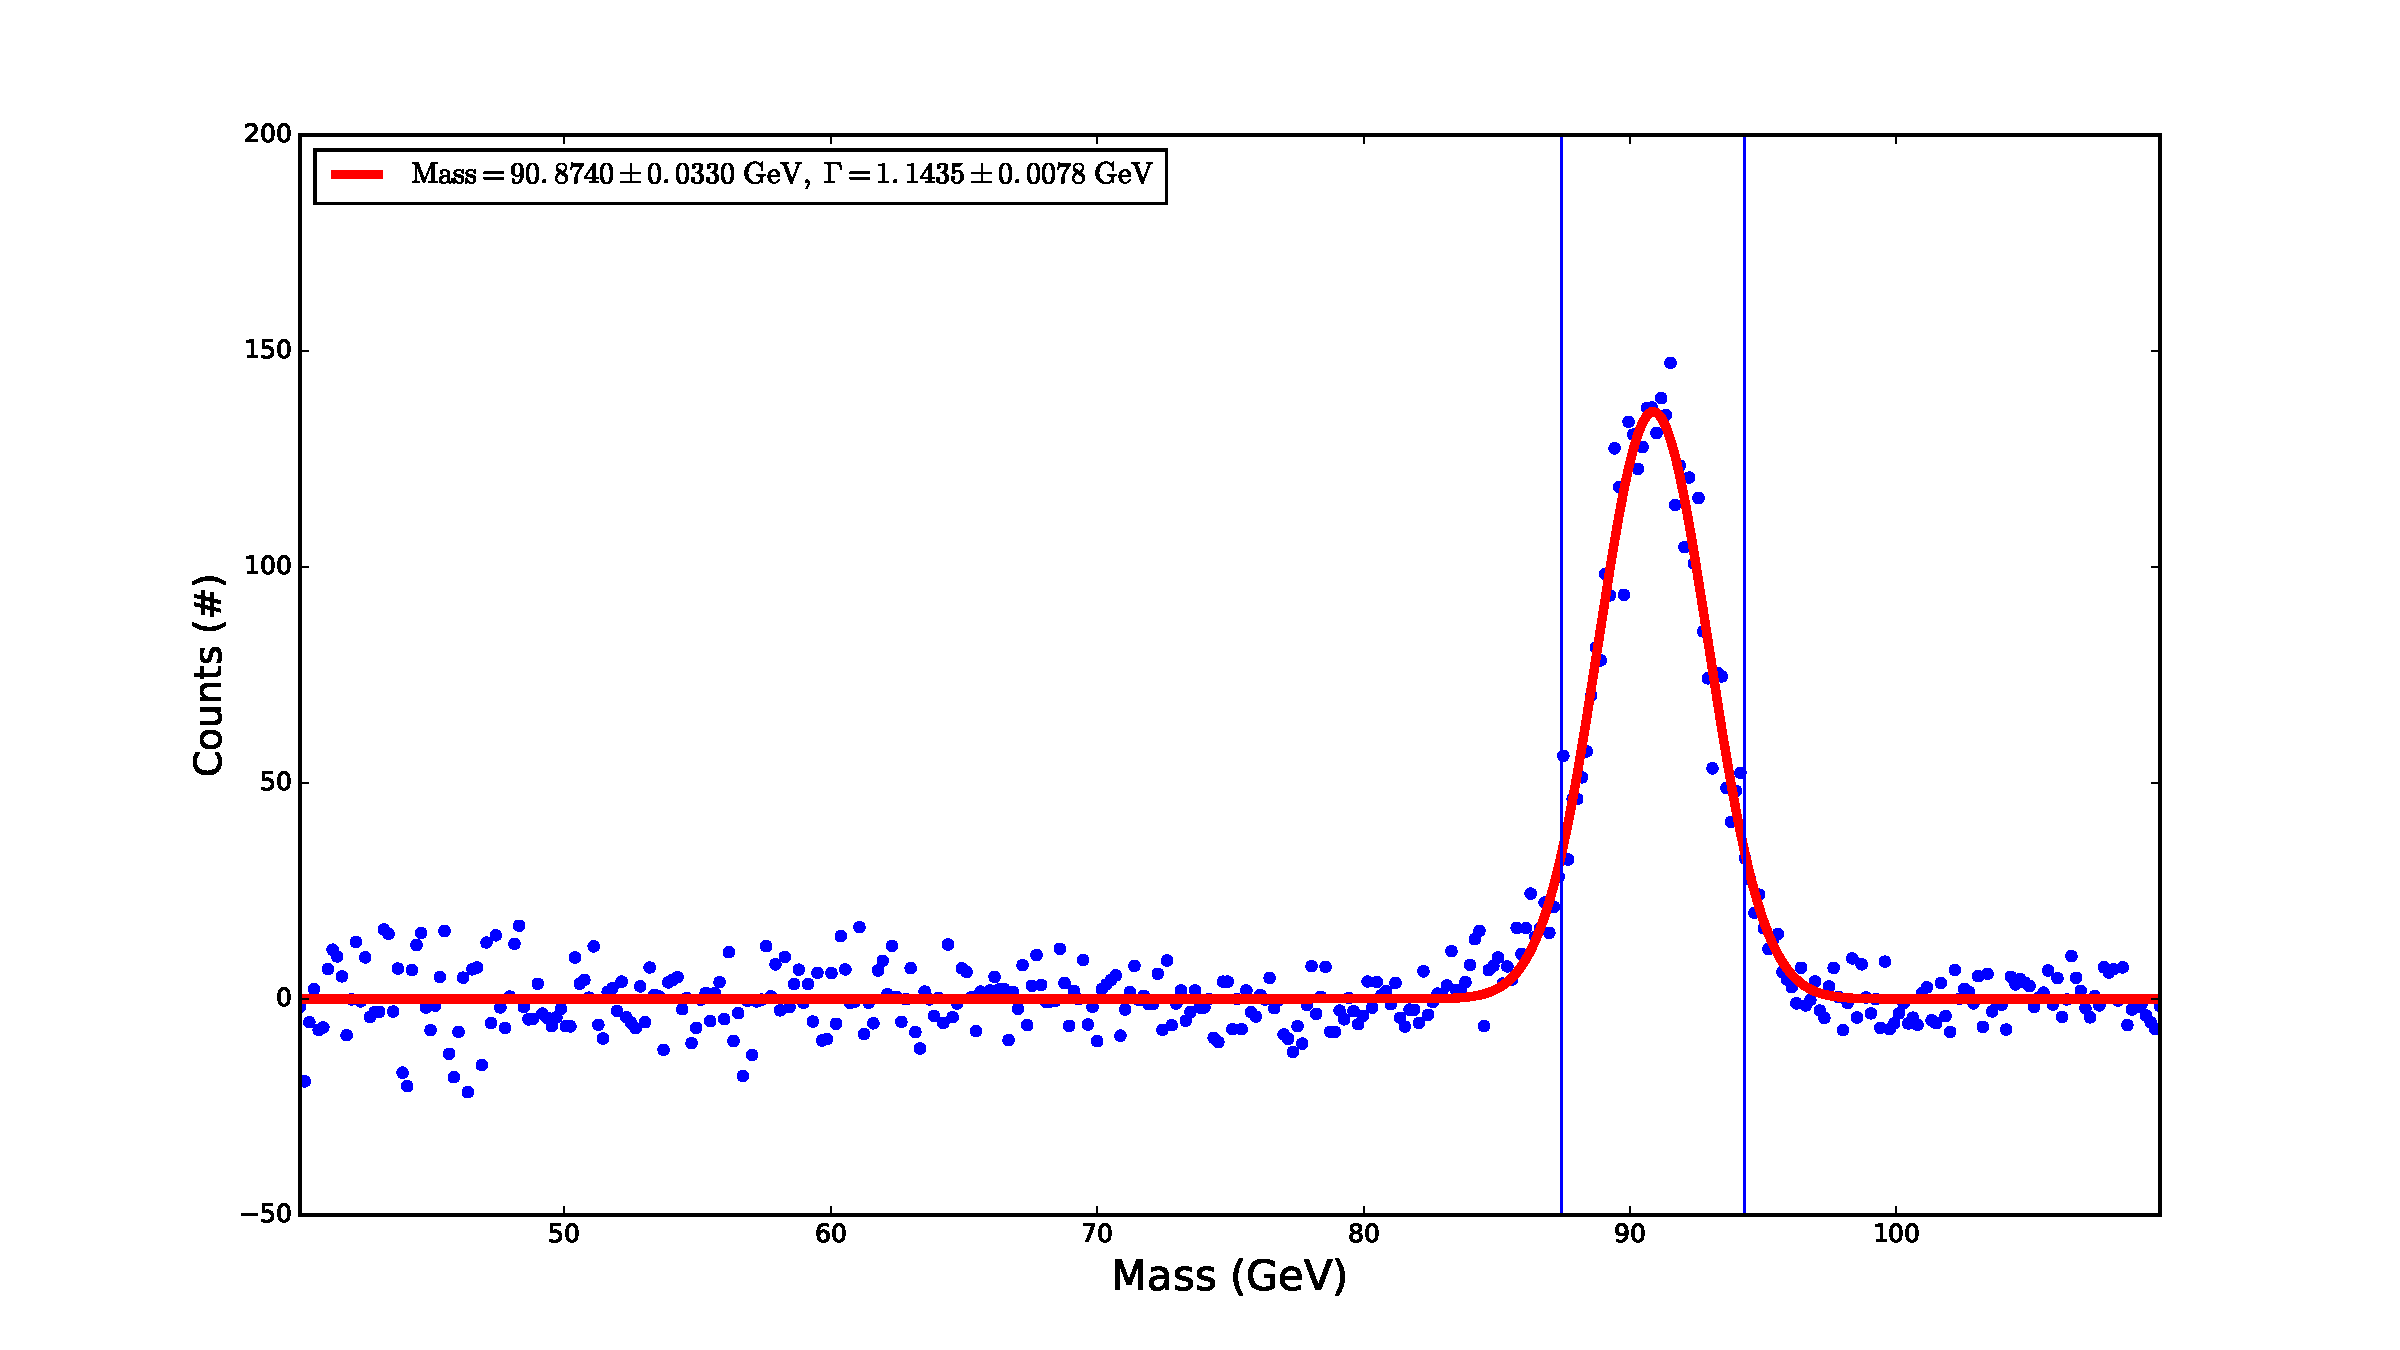
\includegraphics[width=\textwidth]{Z_stuff/Z_peak.pdf} \\

I cut the data around around the mass peak and then looked at different energy and momentum distributions of the decaying $Z^0$.

\subsection*{Scatter Matrix}
The quickest way to find interesting distributions is by looking at the matrix of the scatter plots from different combinations of the energy and momentum directions. \\
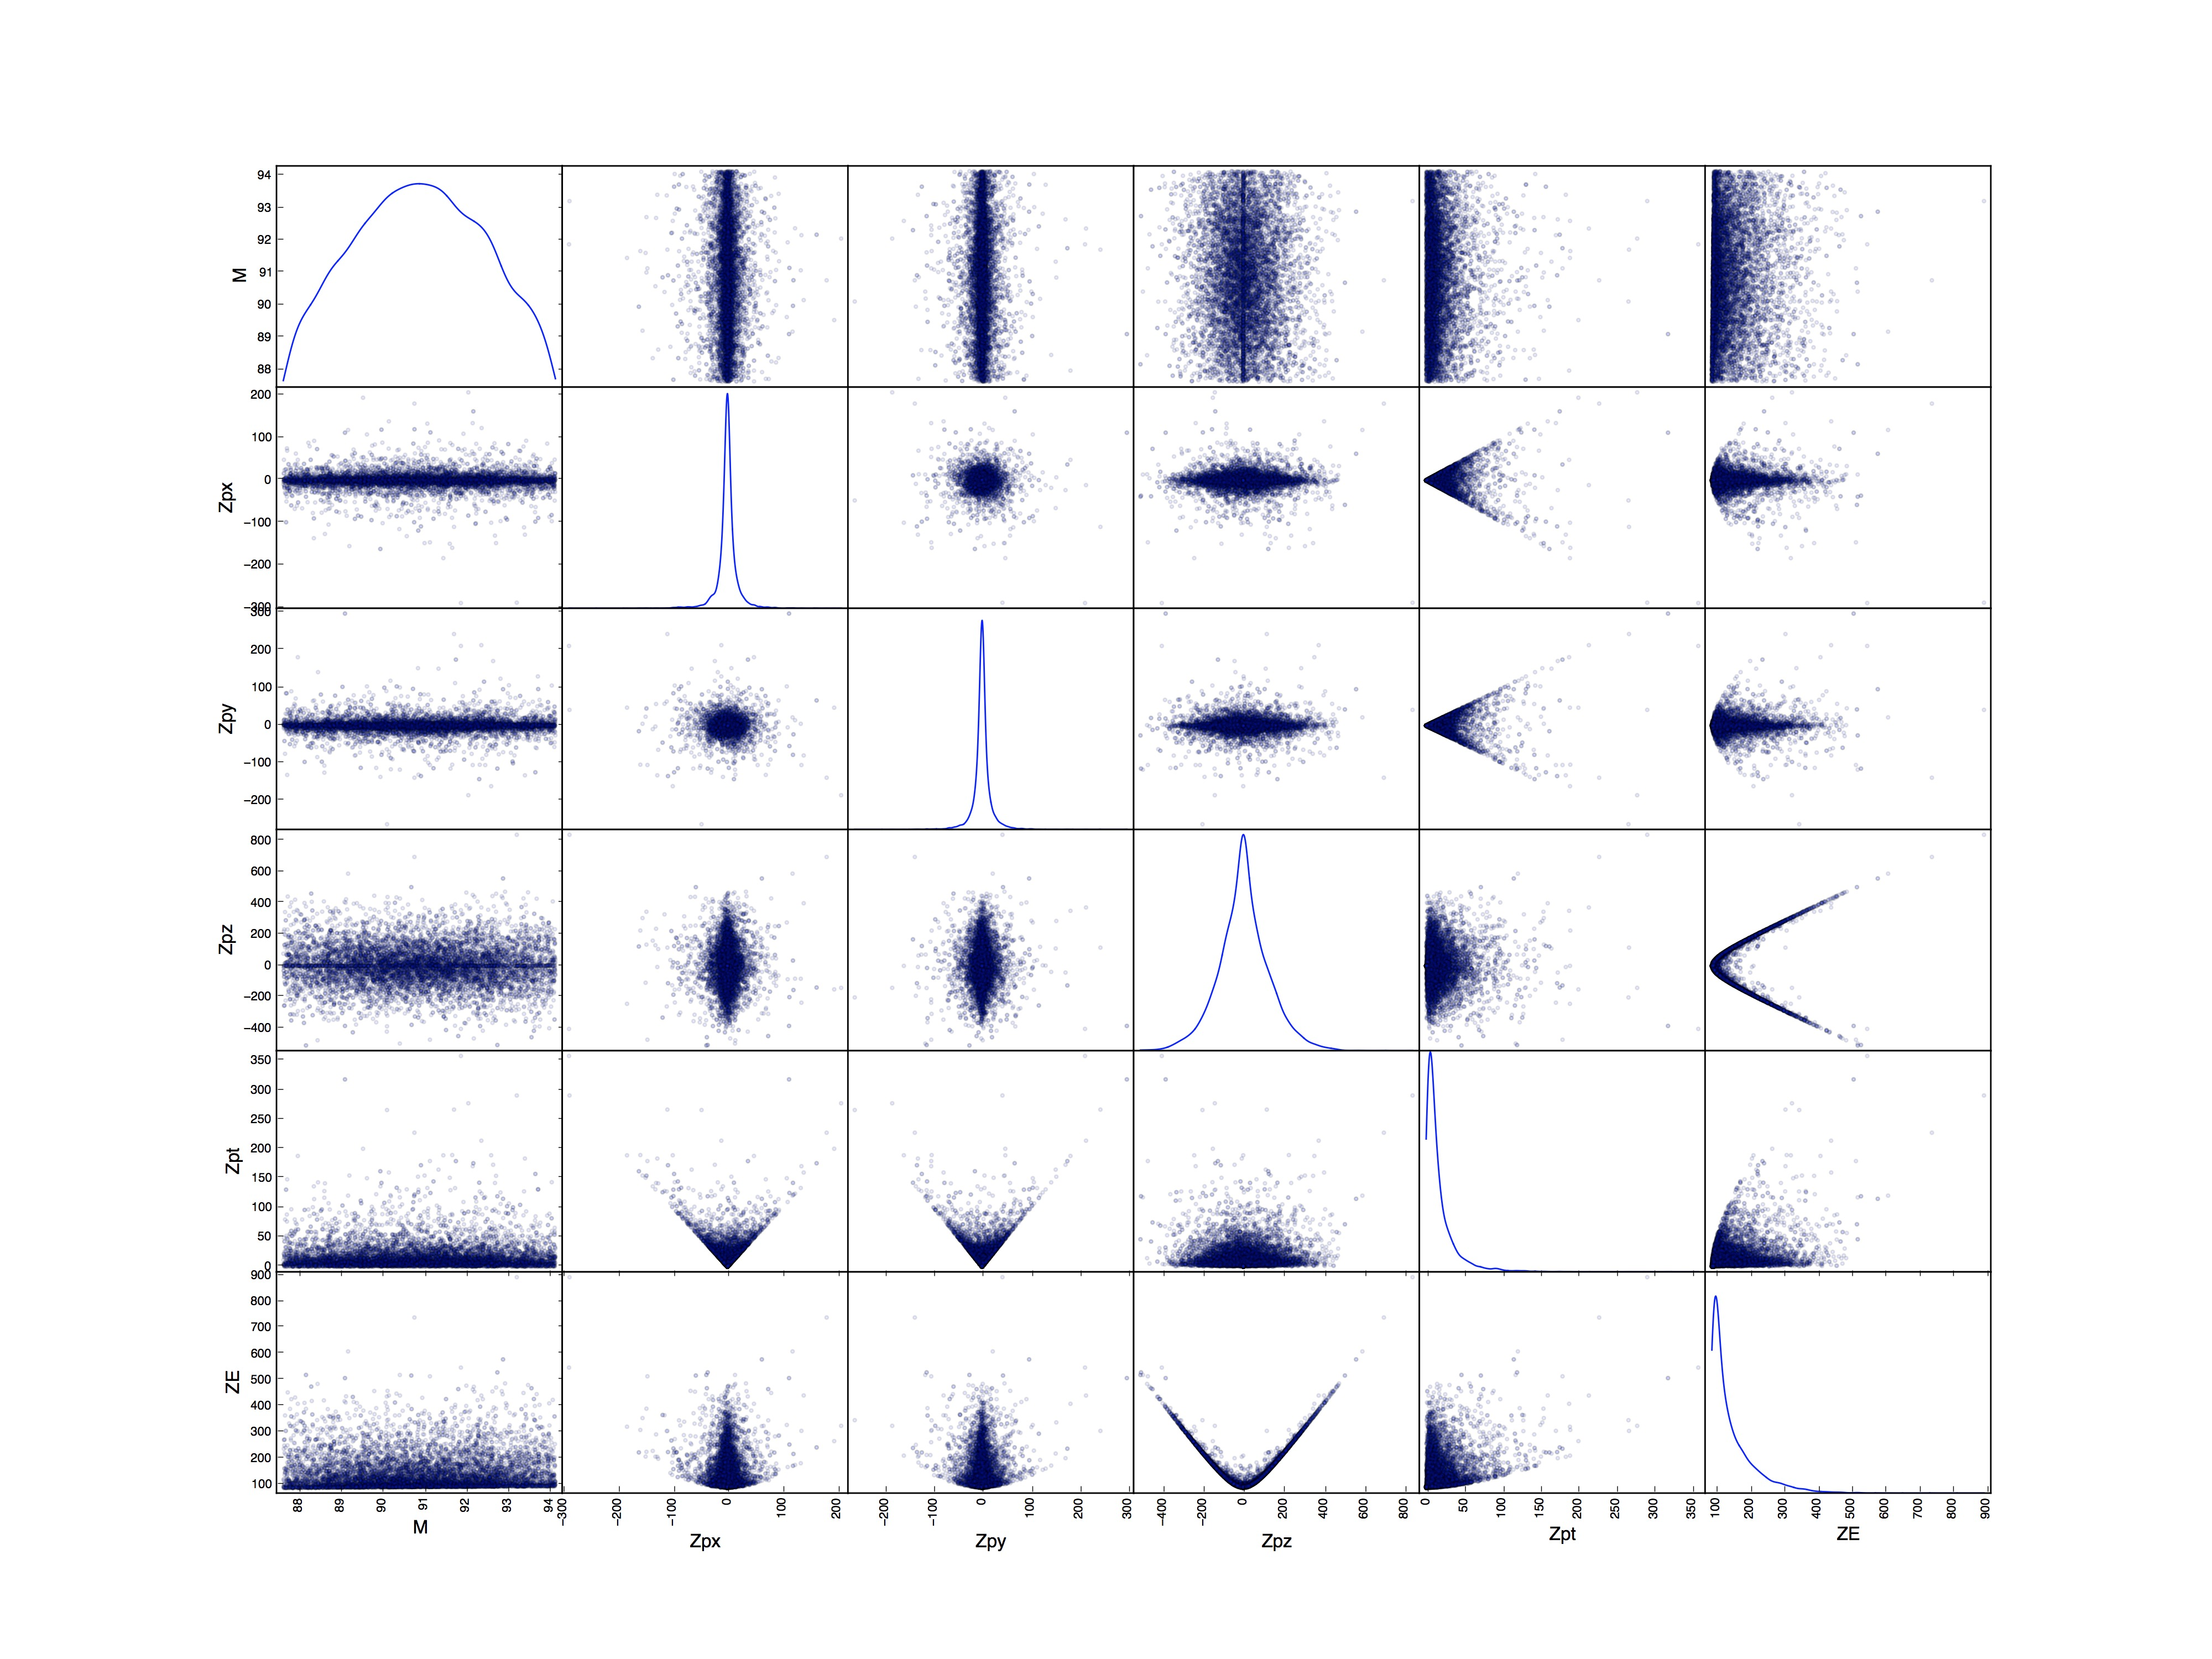
\includegraphics[width=0.9\textwidth]{Z_stuff/scatter_matrix.jpg} \\

The two plots that stick out the most initially are the $Z^0$ Energy versus $Z^0$ Pz and $Z^0$ Energy versus $Z^0$ Pt so I investigated them more. 

\subsection*{$Z^0$ Energy versus $Z^0$ Pz}
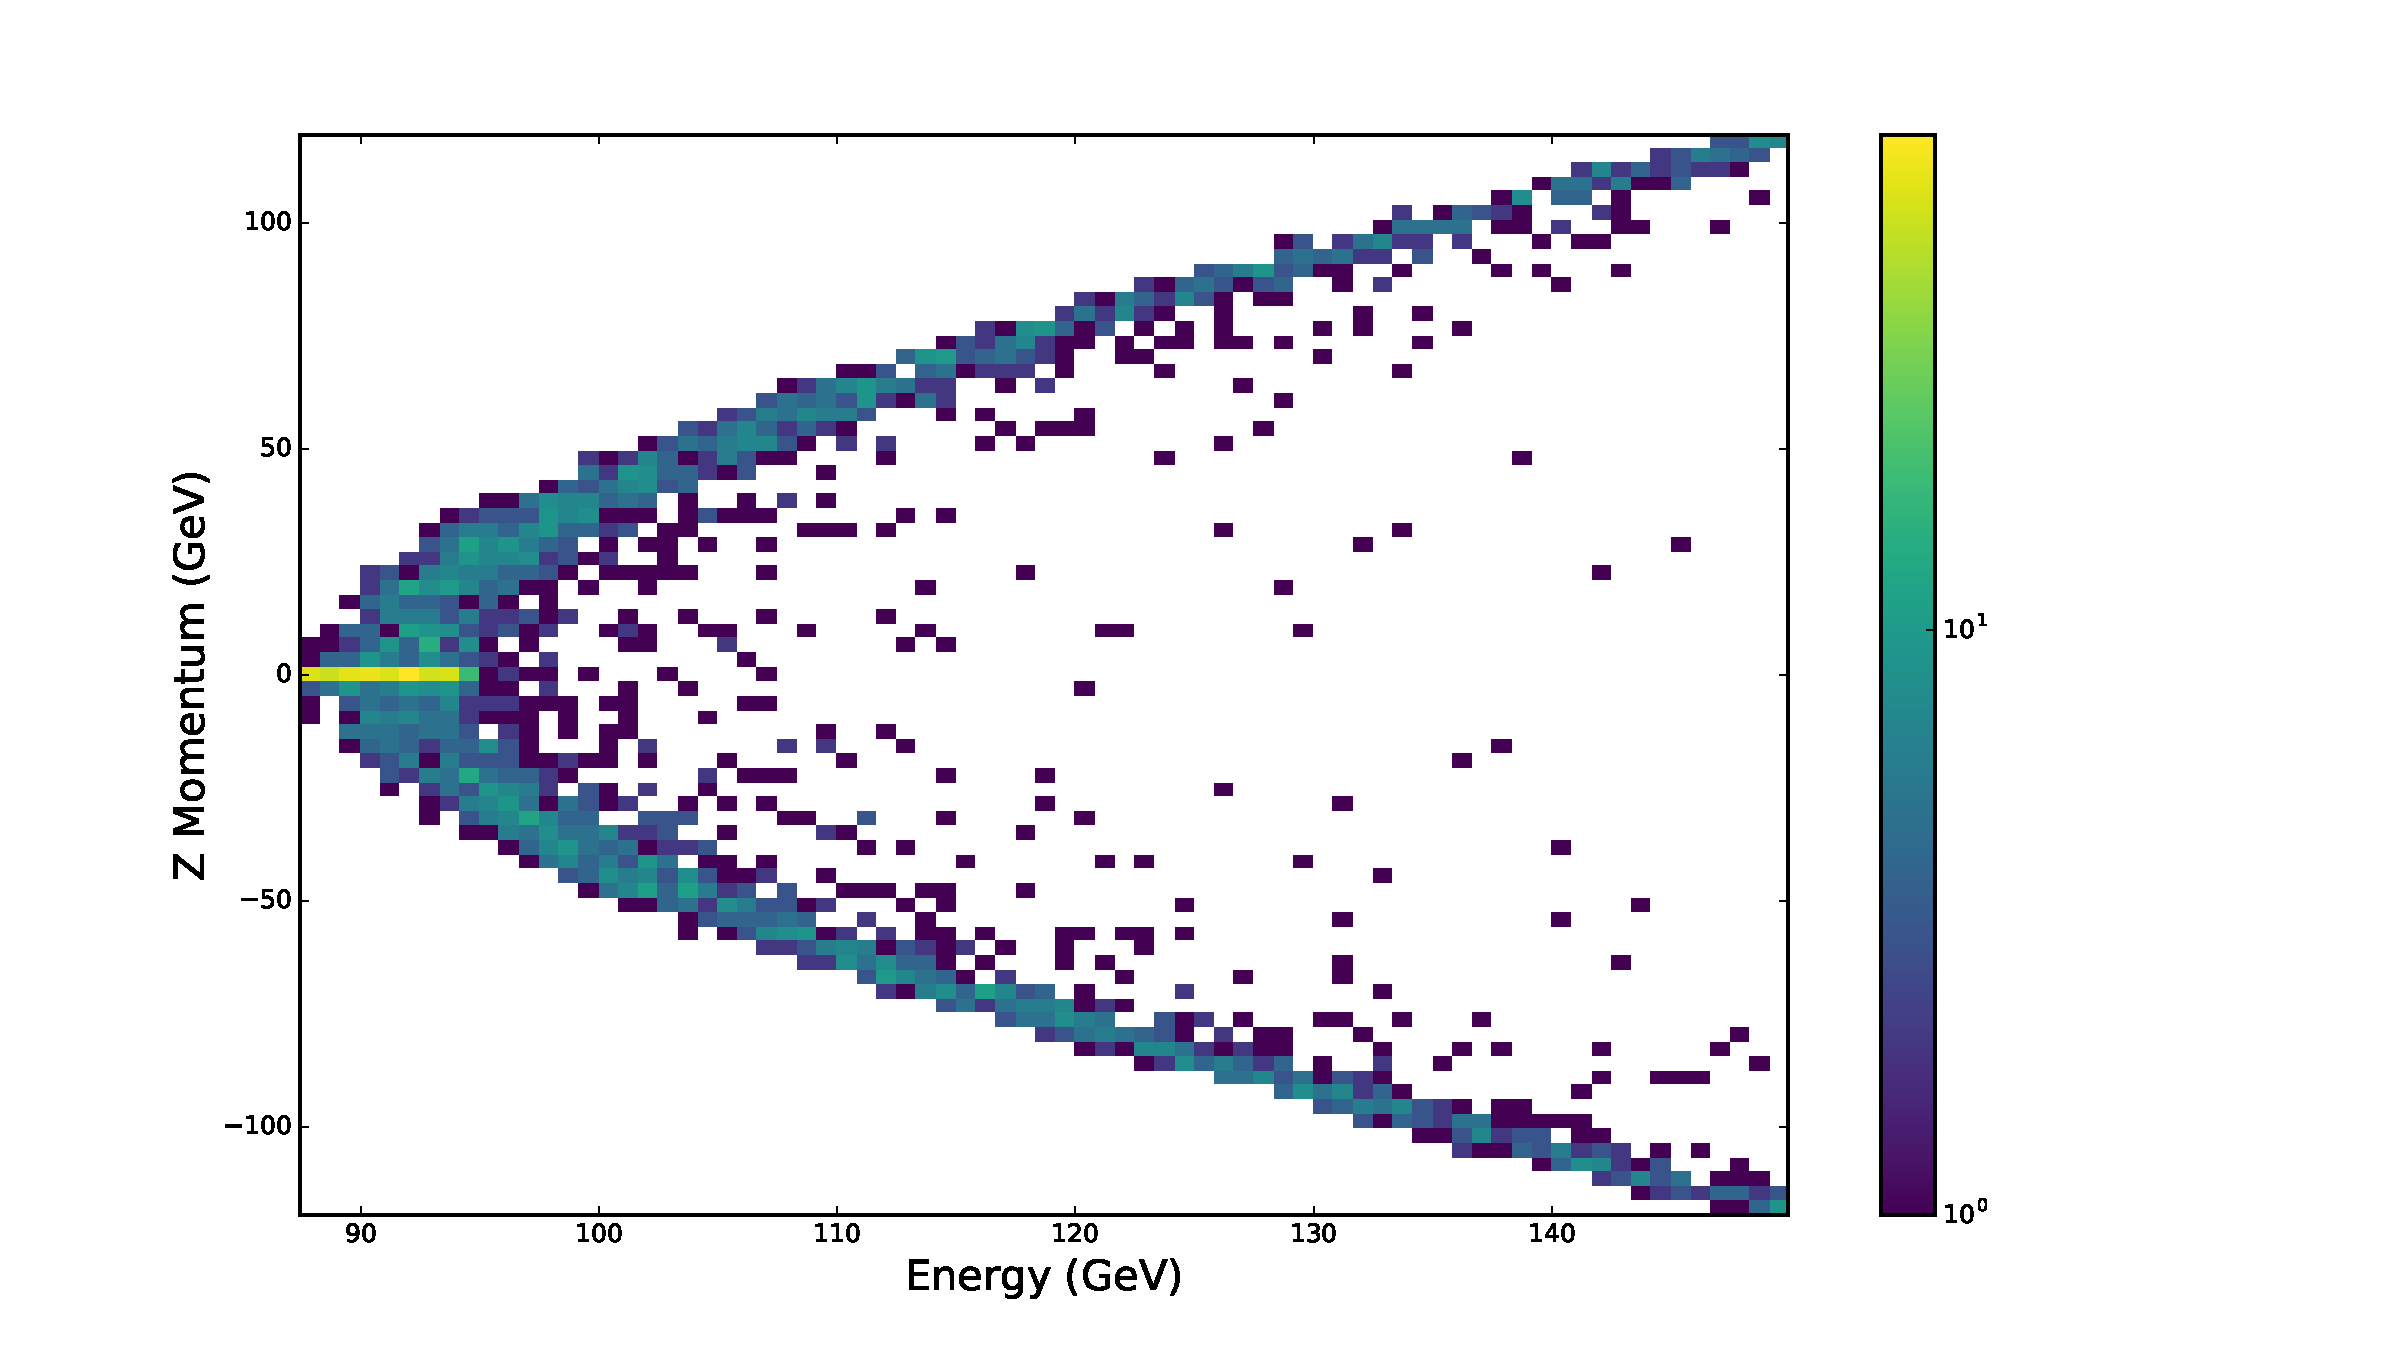
\includegraphics[width=\textwidth]{Z_stuff/ZE_Zpz.pdf} \\

With the color map it is easy to see that most of the $Z^0$ have close to 0 momentum in the direction of the beam and that they are produced at energies close to $90\,GeV$.  This is characteristic of a symmetric beam collider like the LHC where particles are created close to the center of the lab frame. By looking at the projection along the Z momentum axis it's clear to see this large peak of $Pz \approx 0$. \\

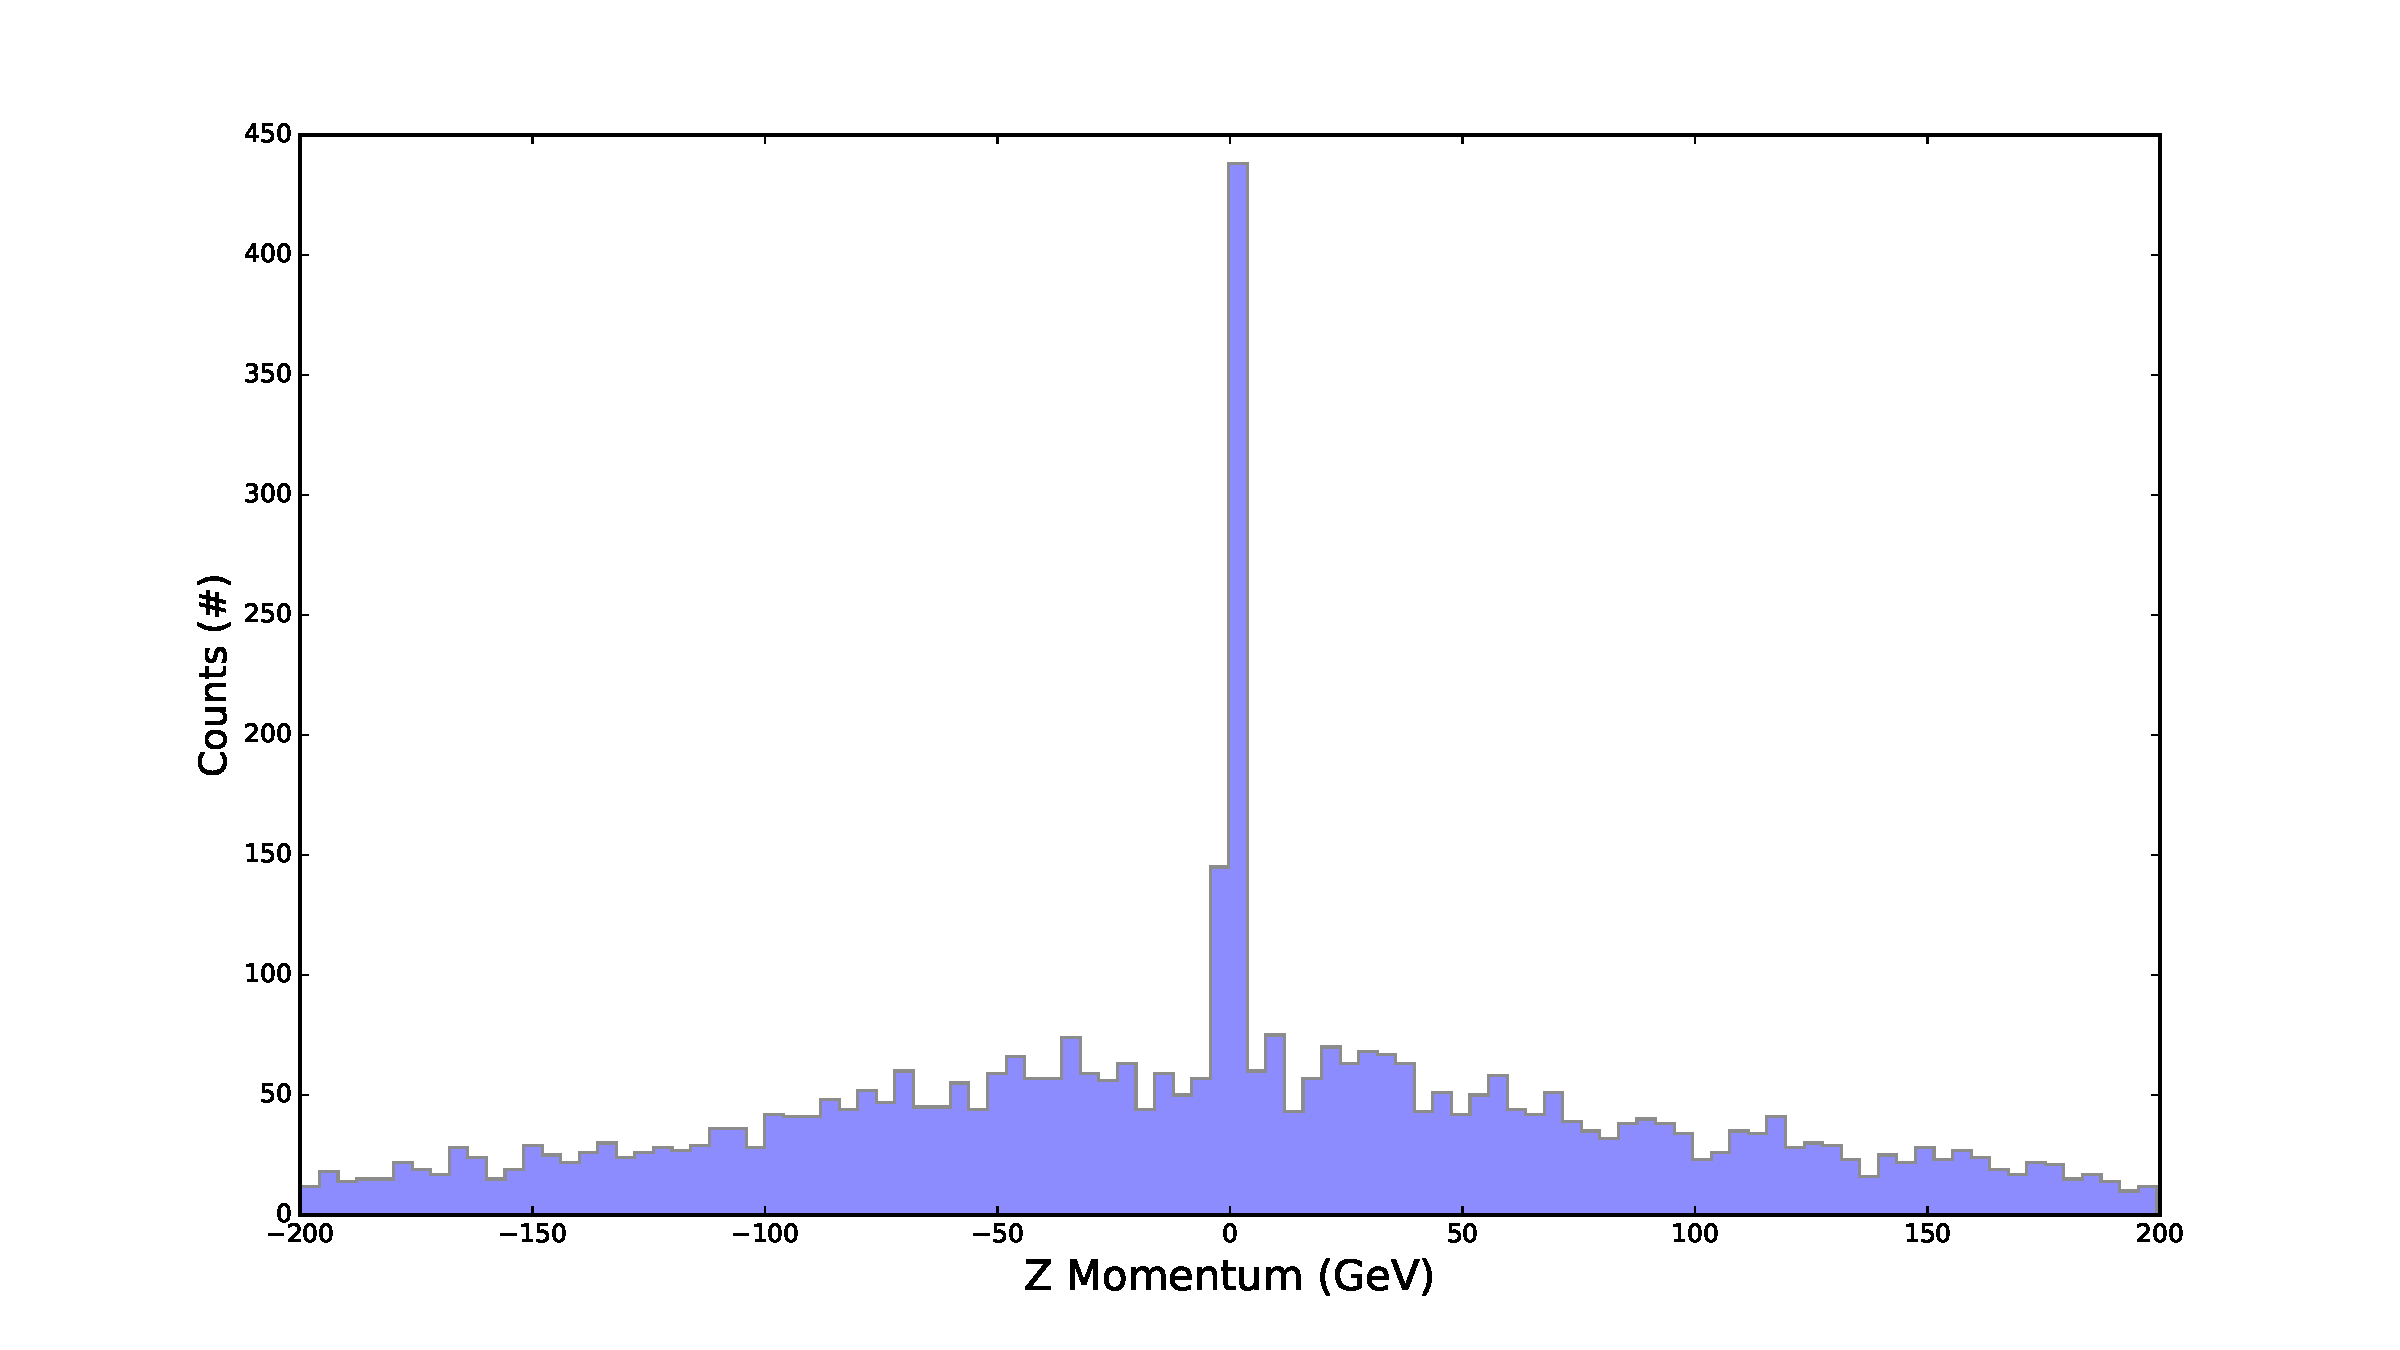
\includegraphics[width=\textwidth]{Z_stuff/Zpz.pdf} \\

There is a large peak around 0 with a very small distribution at larger momentums.

\subsection*{$Z^0$ Energy versus $Z^0$ Pt}
Another interesting distribution is the $Z^0$ Energy versus $Z^0$ transverse momentum. This graph also shows that a large amount of the $Z^0$ have $Pz \approx 0$ \\
\includegraphics[width=\textwidth]{Z_stuff/ZE_Zpt_log.pdf} \\

Looking at the projection along Pt confirms this. \\ 
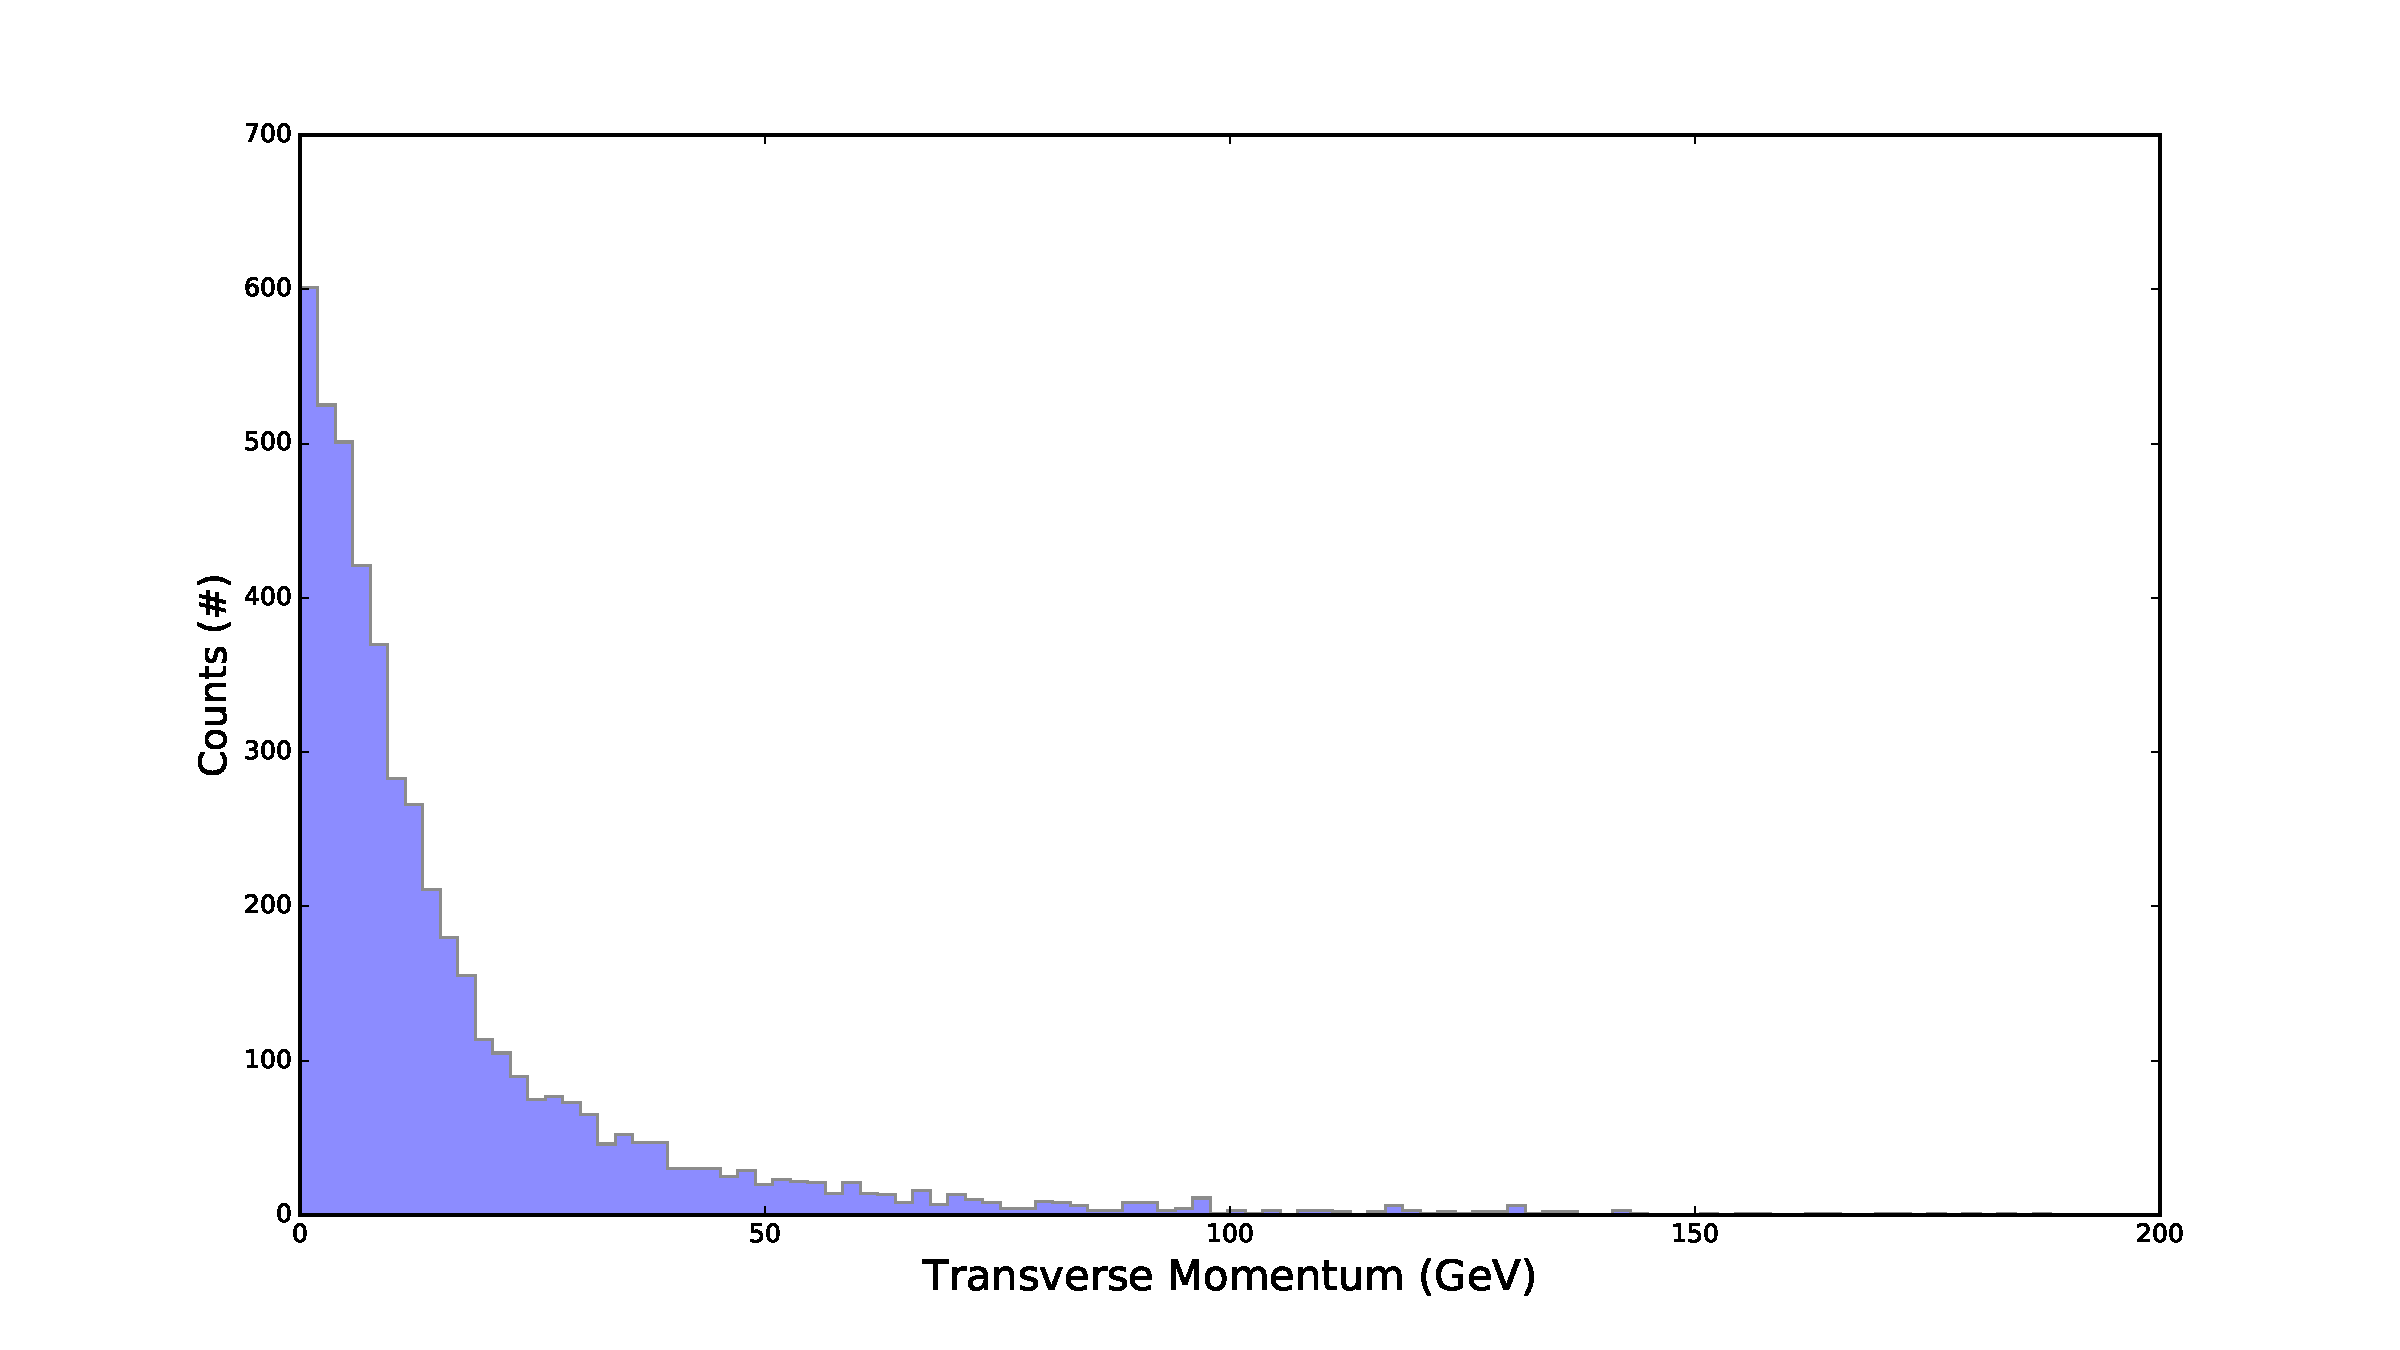
\includegraphics[width=\textwidth]{Z_stuff/Zpt.pdf} \\

Combining the results from the two investigations and looking at the $Z^0$ Pz versus $Z^0$ Pt shows that most of the $Z^0$ have $P_{total} \approx 0$ meaning that many of the $Z^0$ are created close to rest in the lab frame.  This means that they will decay very quickly and that the decaying particles will have opposite momentums as they leave the center of the detector region.  This could be helpful in creating a true background subtraction to find $Z^0$ for this experiment by only selecting decays which come from the close to the center of the detector and have $P_{total} \approx 0$ within detector resolutions. \\

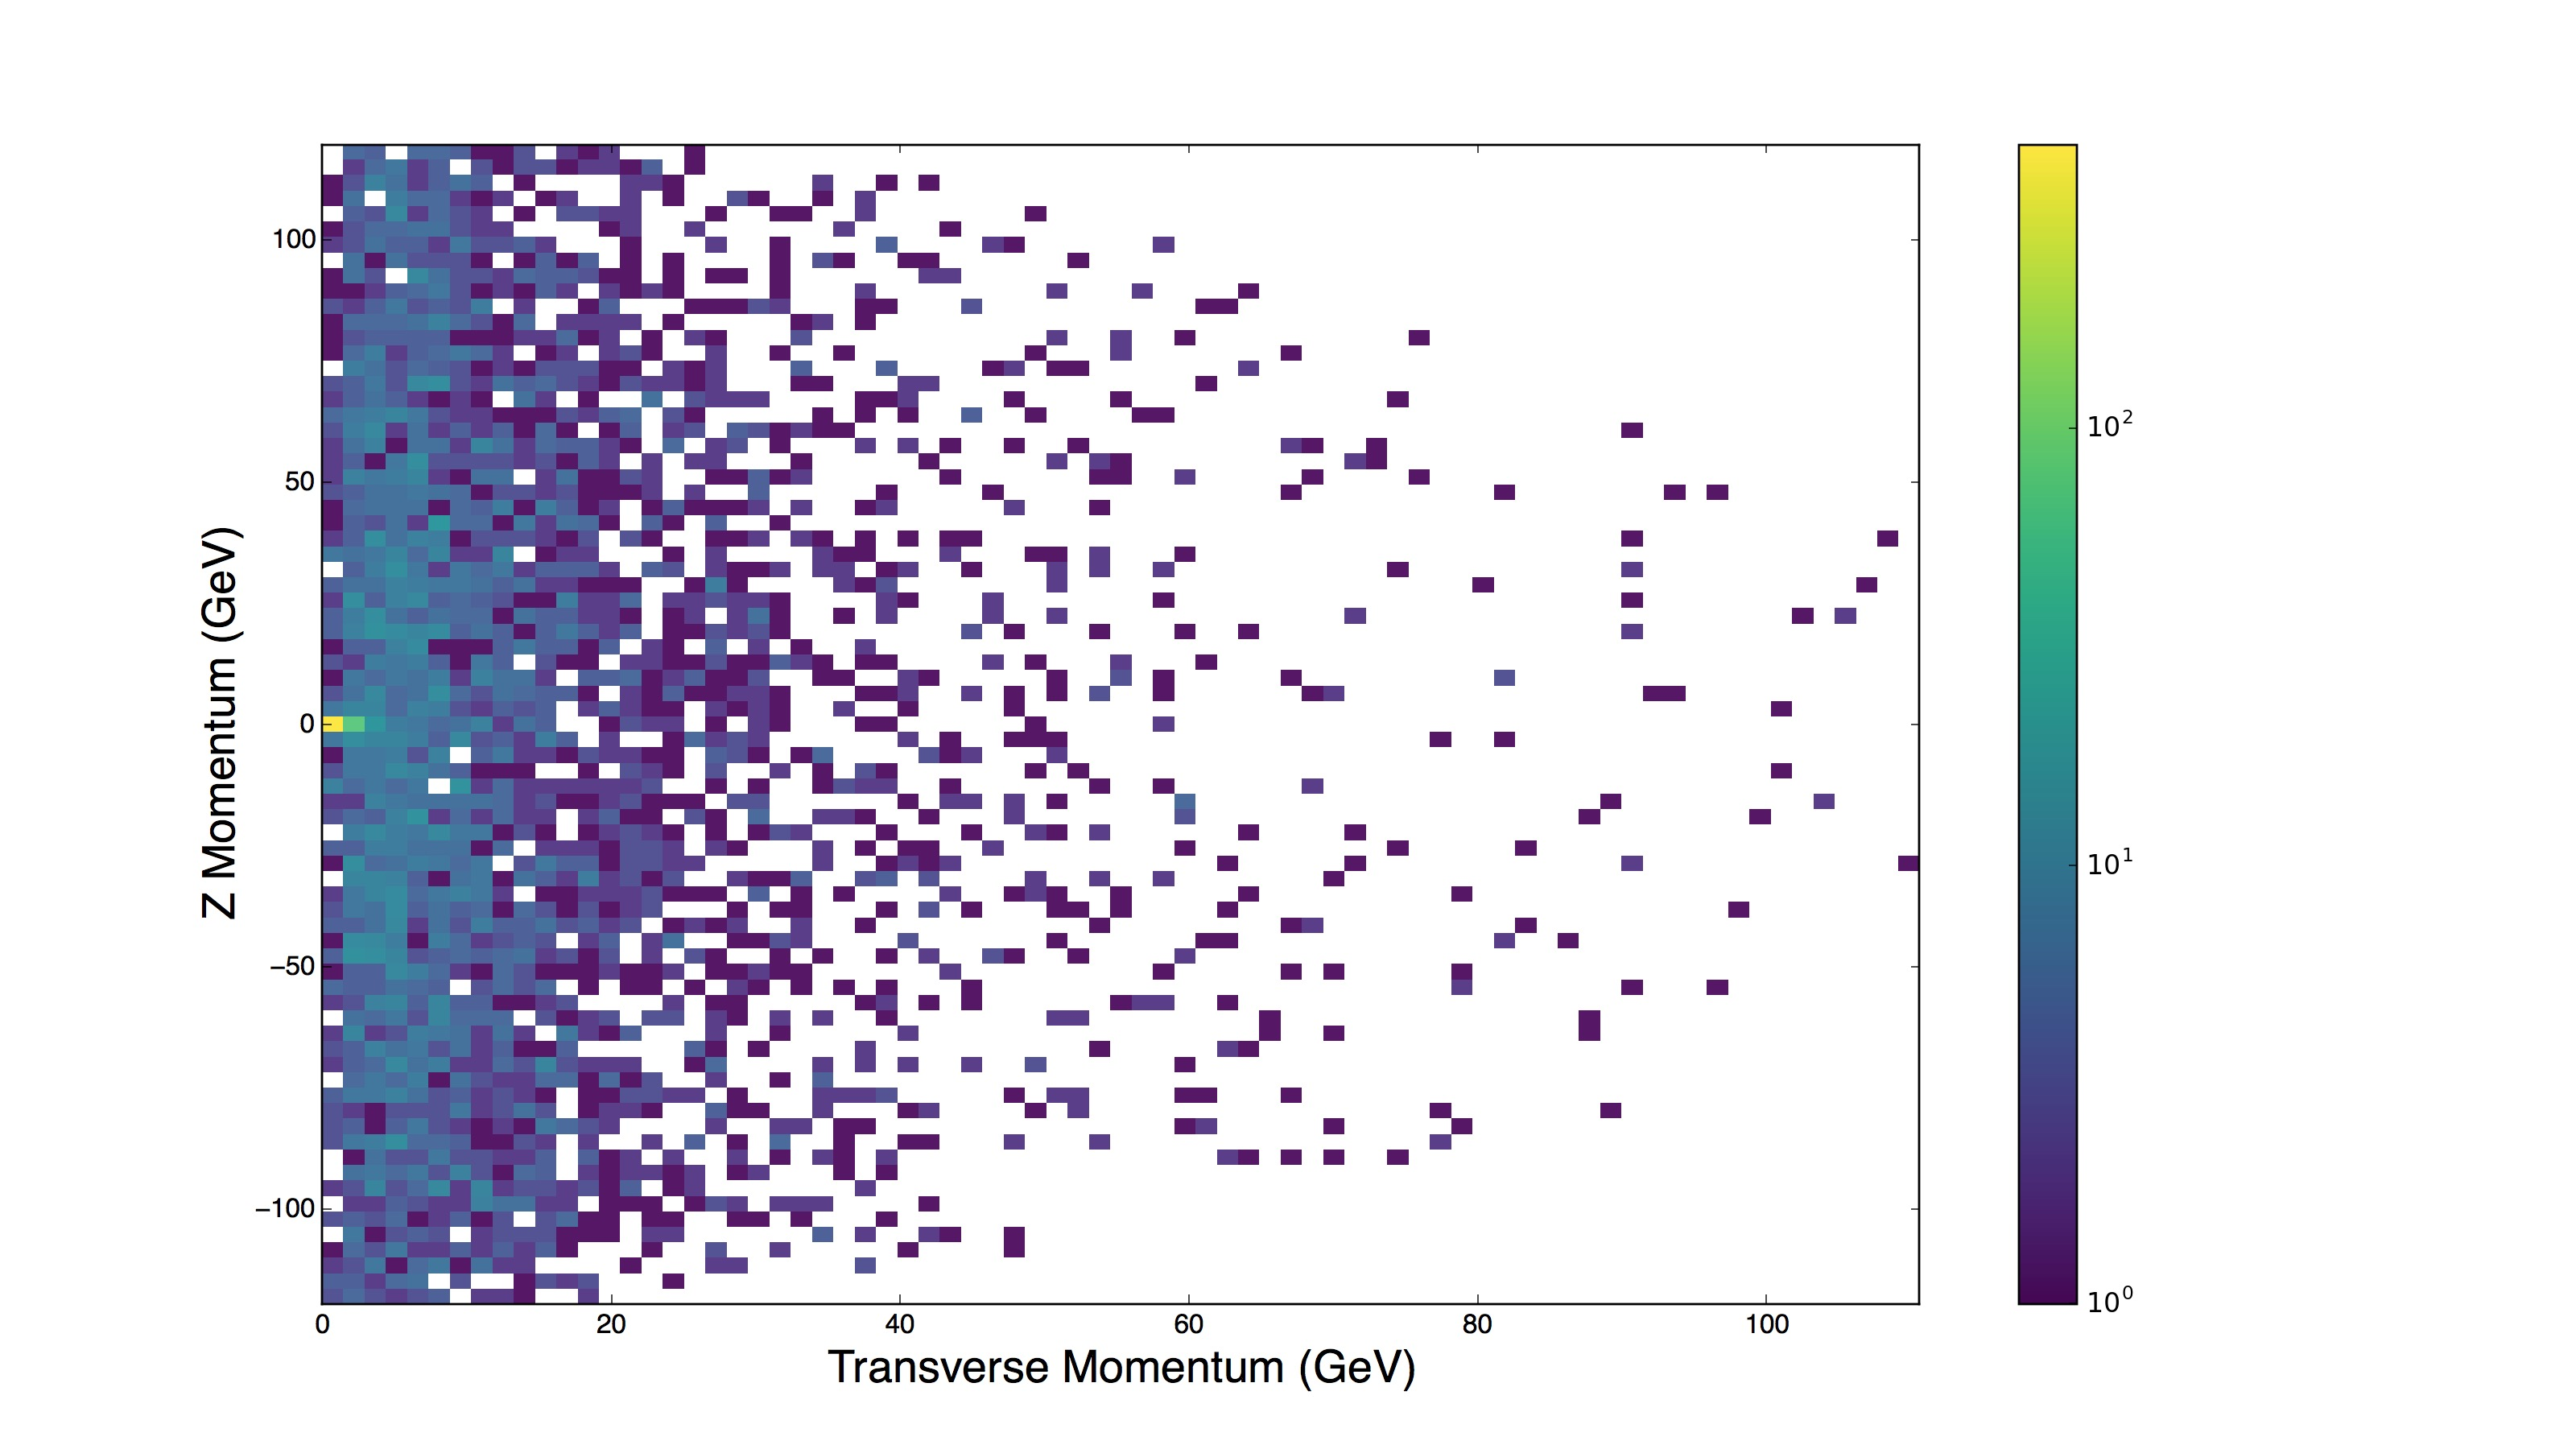
\includegraphics[width=\textwidth]{Z_stuff/Zpt_Zpz.pdf} \\

\section*{$\Upsilon$ Decays}

The next region I looked at was the region between $6 - 14\,GeV$ where the $\Upsilon$ can be found. Again I looked at the mass histogram and fit a polynomial background with a Gaussian peak this time around $9.45\,GeV$. The $\chi^2$ for this distribution is much larger than in the $Z^0$ case because there are two peaks which are not initially fit but the Gaussian or the polynomial. \\

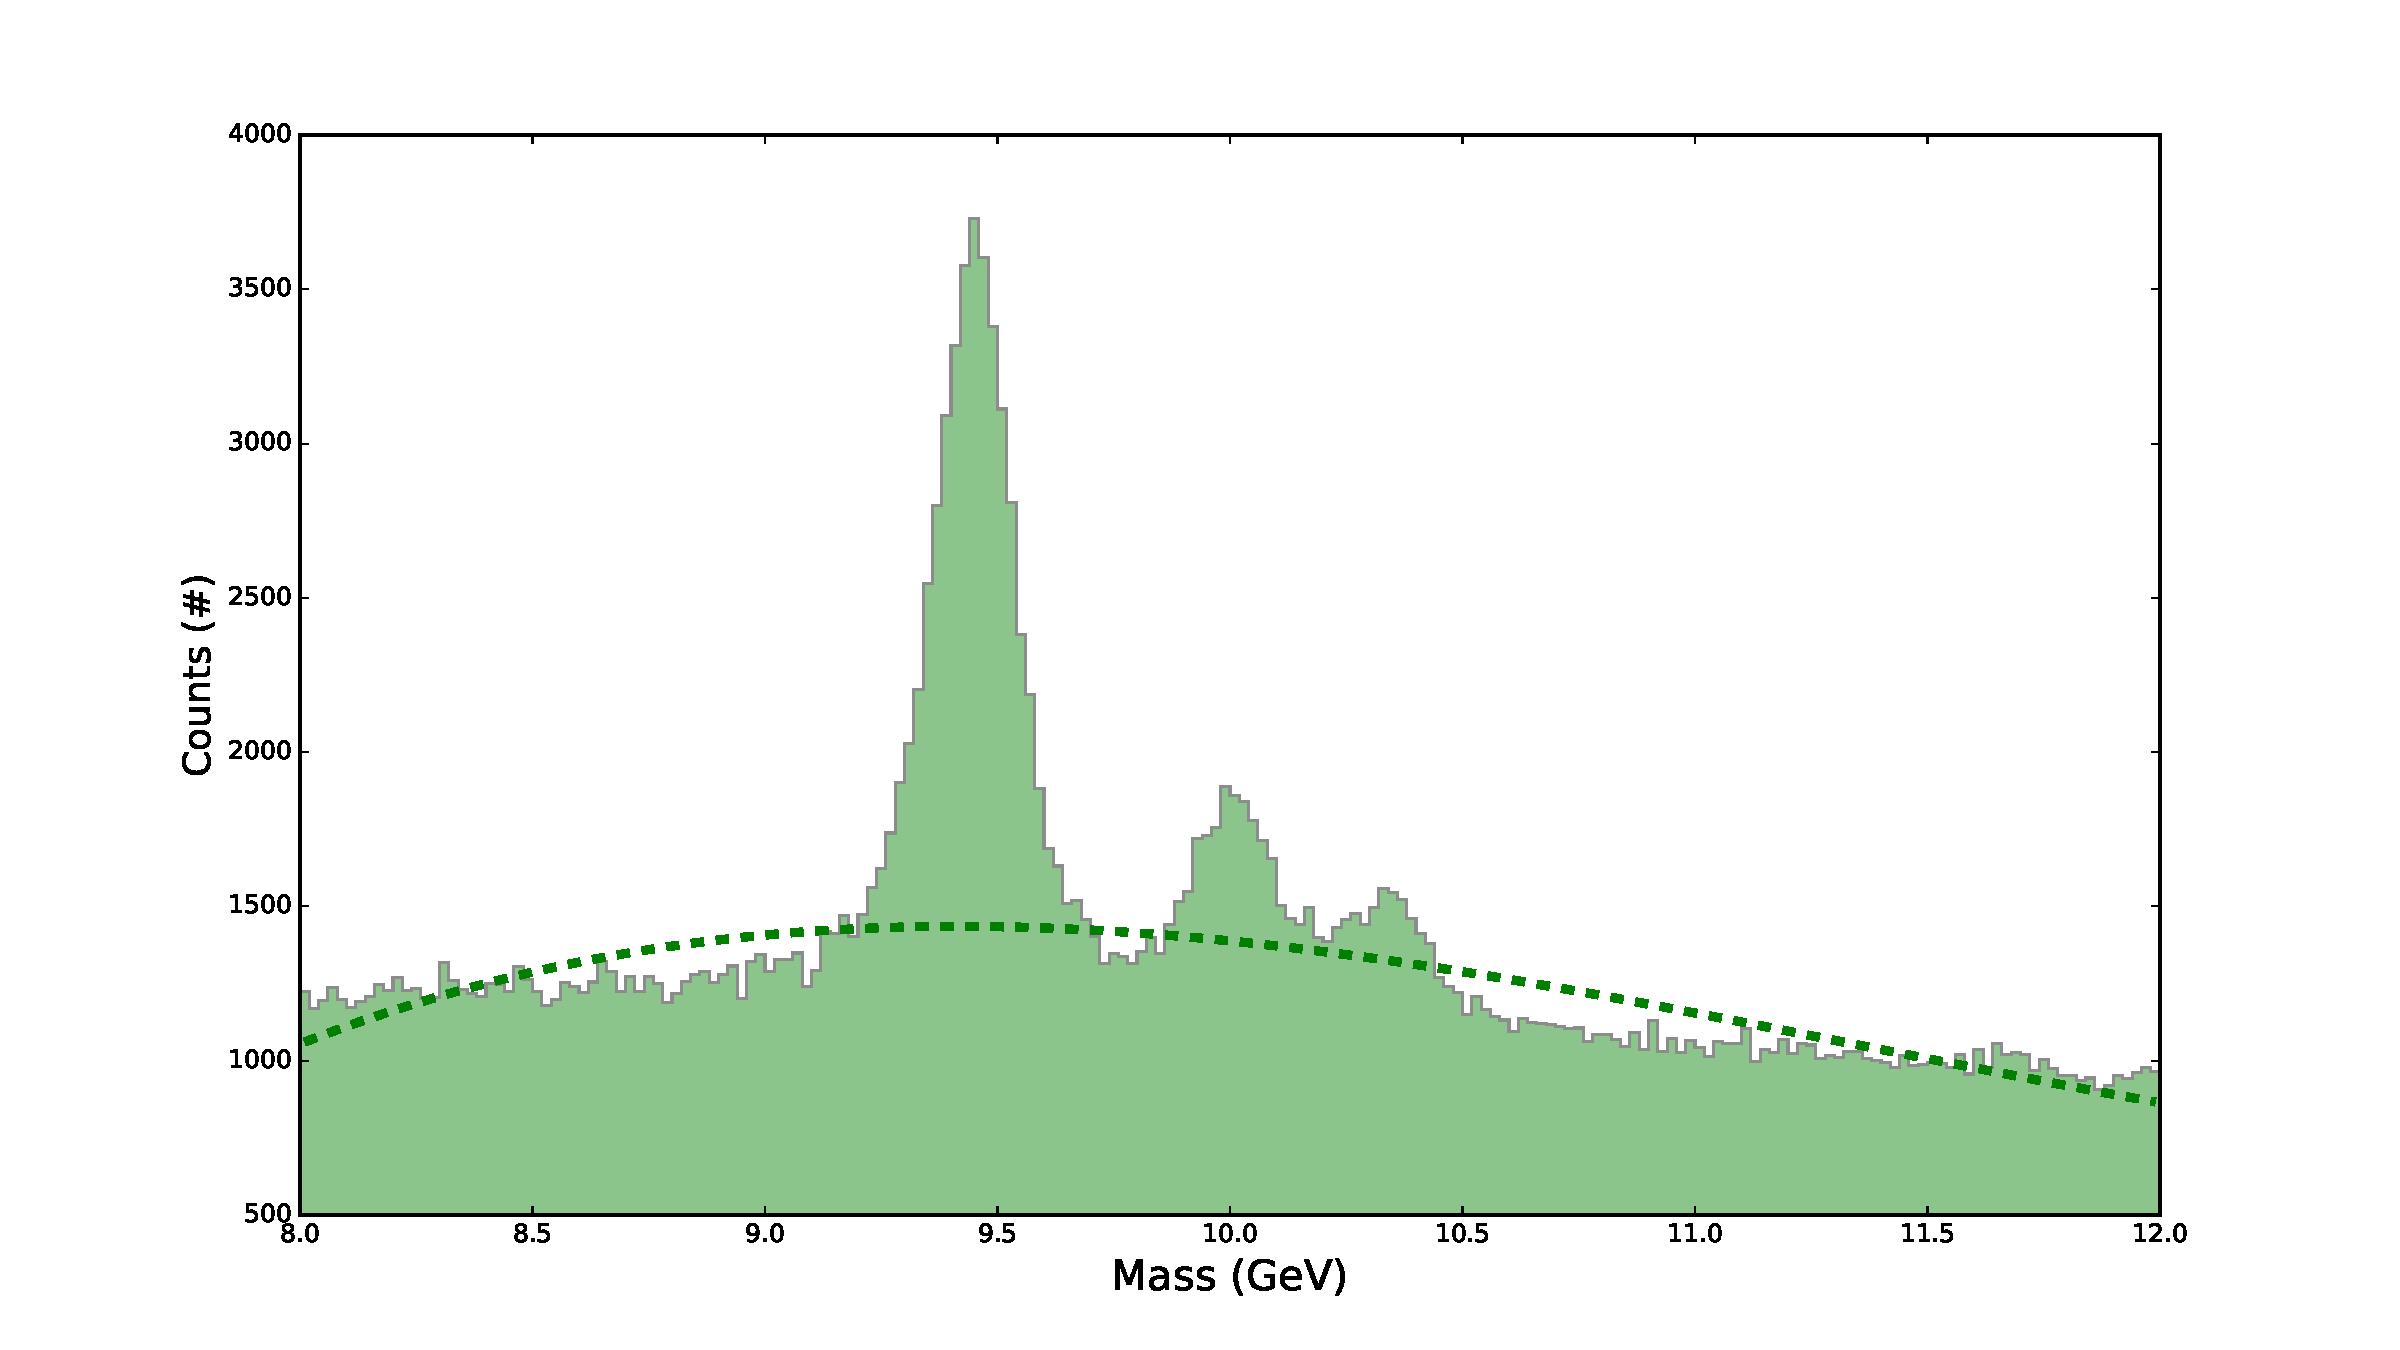
\includegraphics[width=\textwidth]{Upsilon/U_hist.pdf} \\

I again subtracted the polynomial background to get the larger peak seen in green.\\

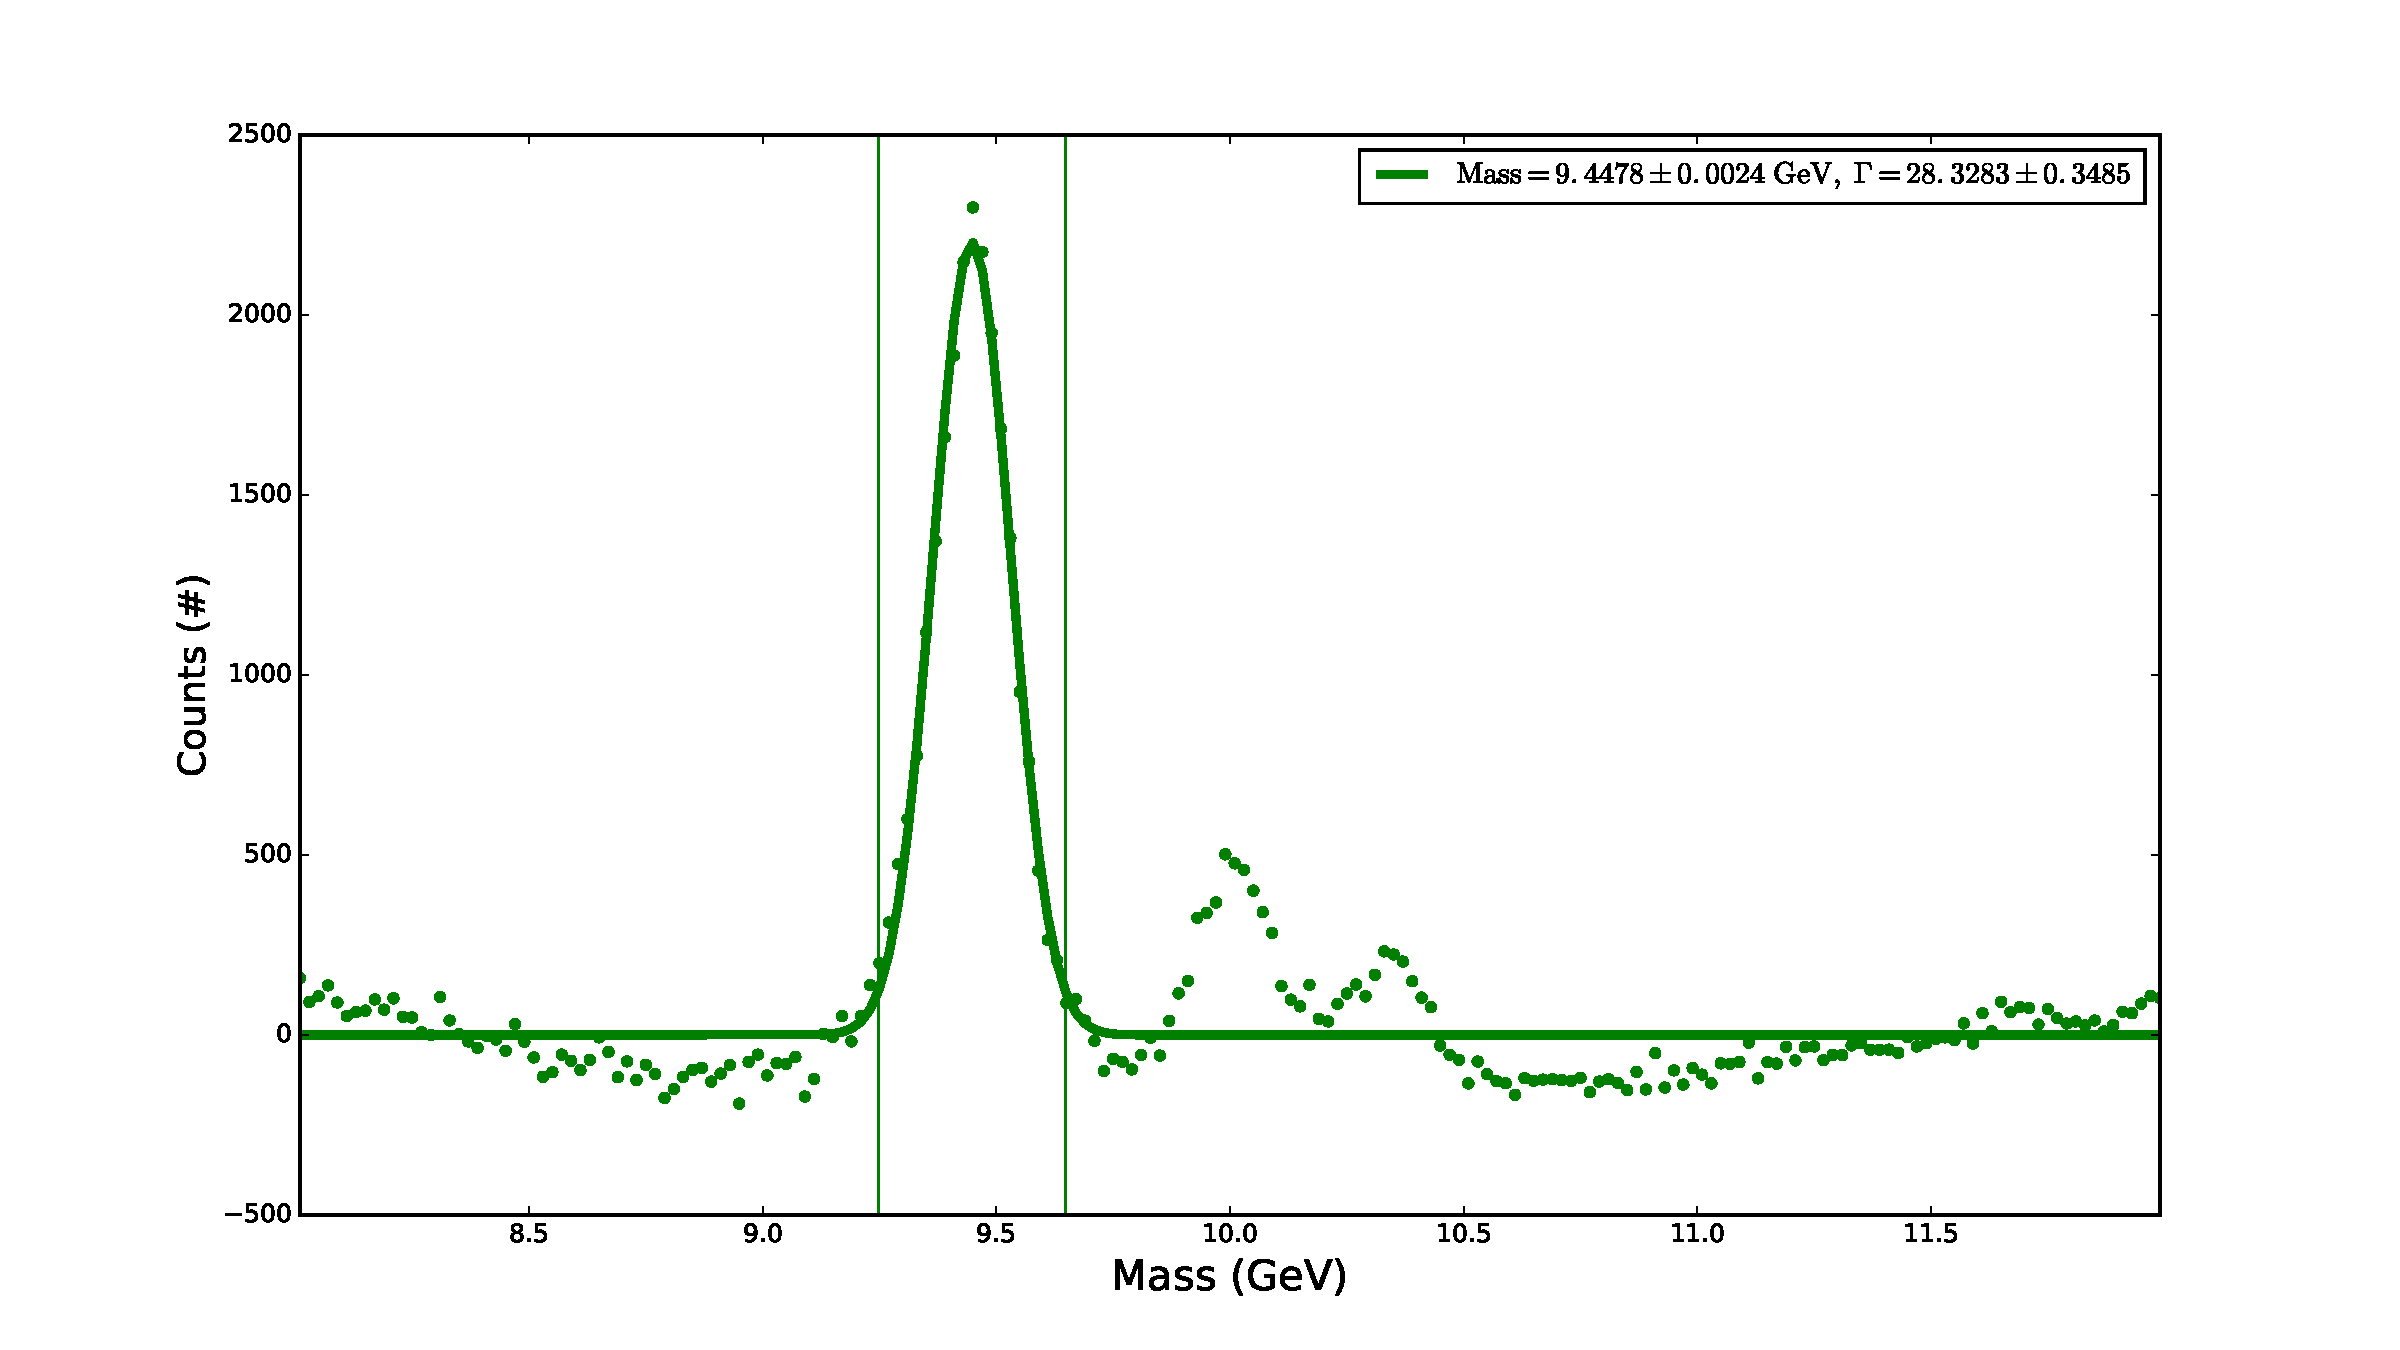
\includegraphics[width=\textwidth]{Upsilon/U_peak.pdf} \\

And then after subtracting the background and the larger of the three peaks I tried to fit the smaller peaks but the simple Gaussian fit method lumped the two remaining peaks together making it hard to distinguish between the two.

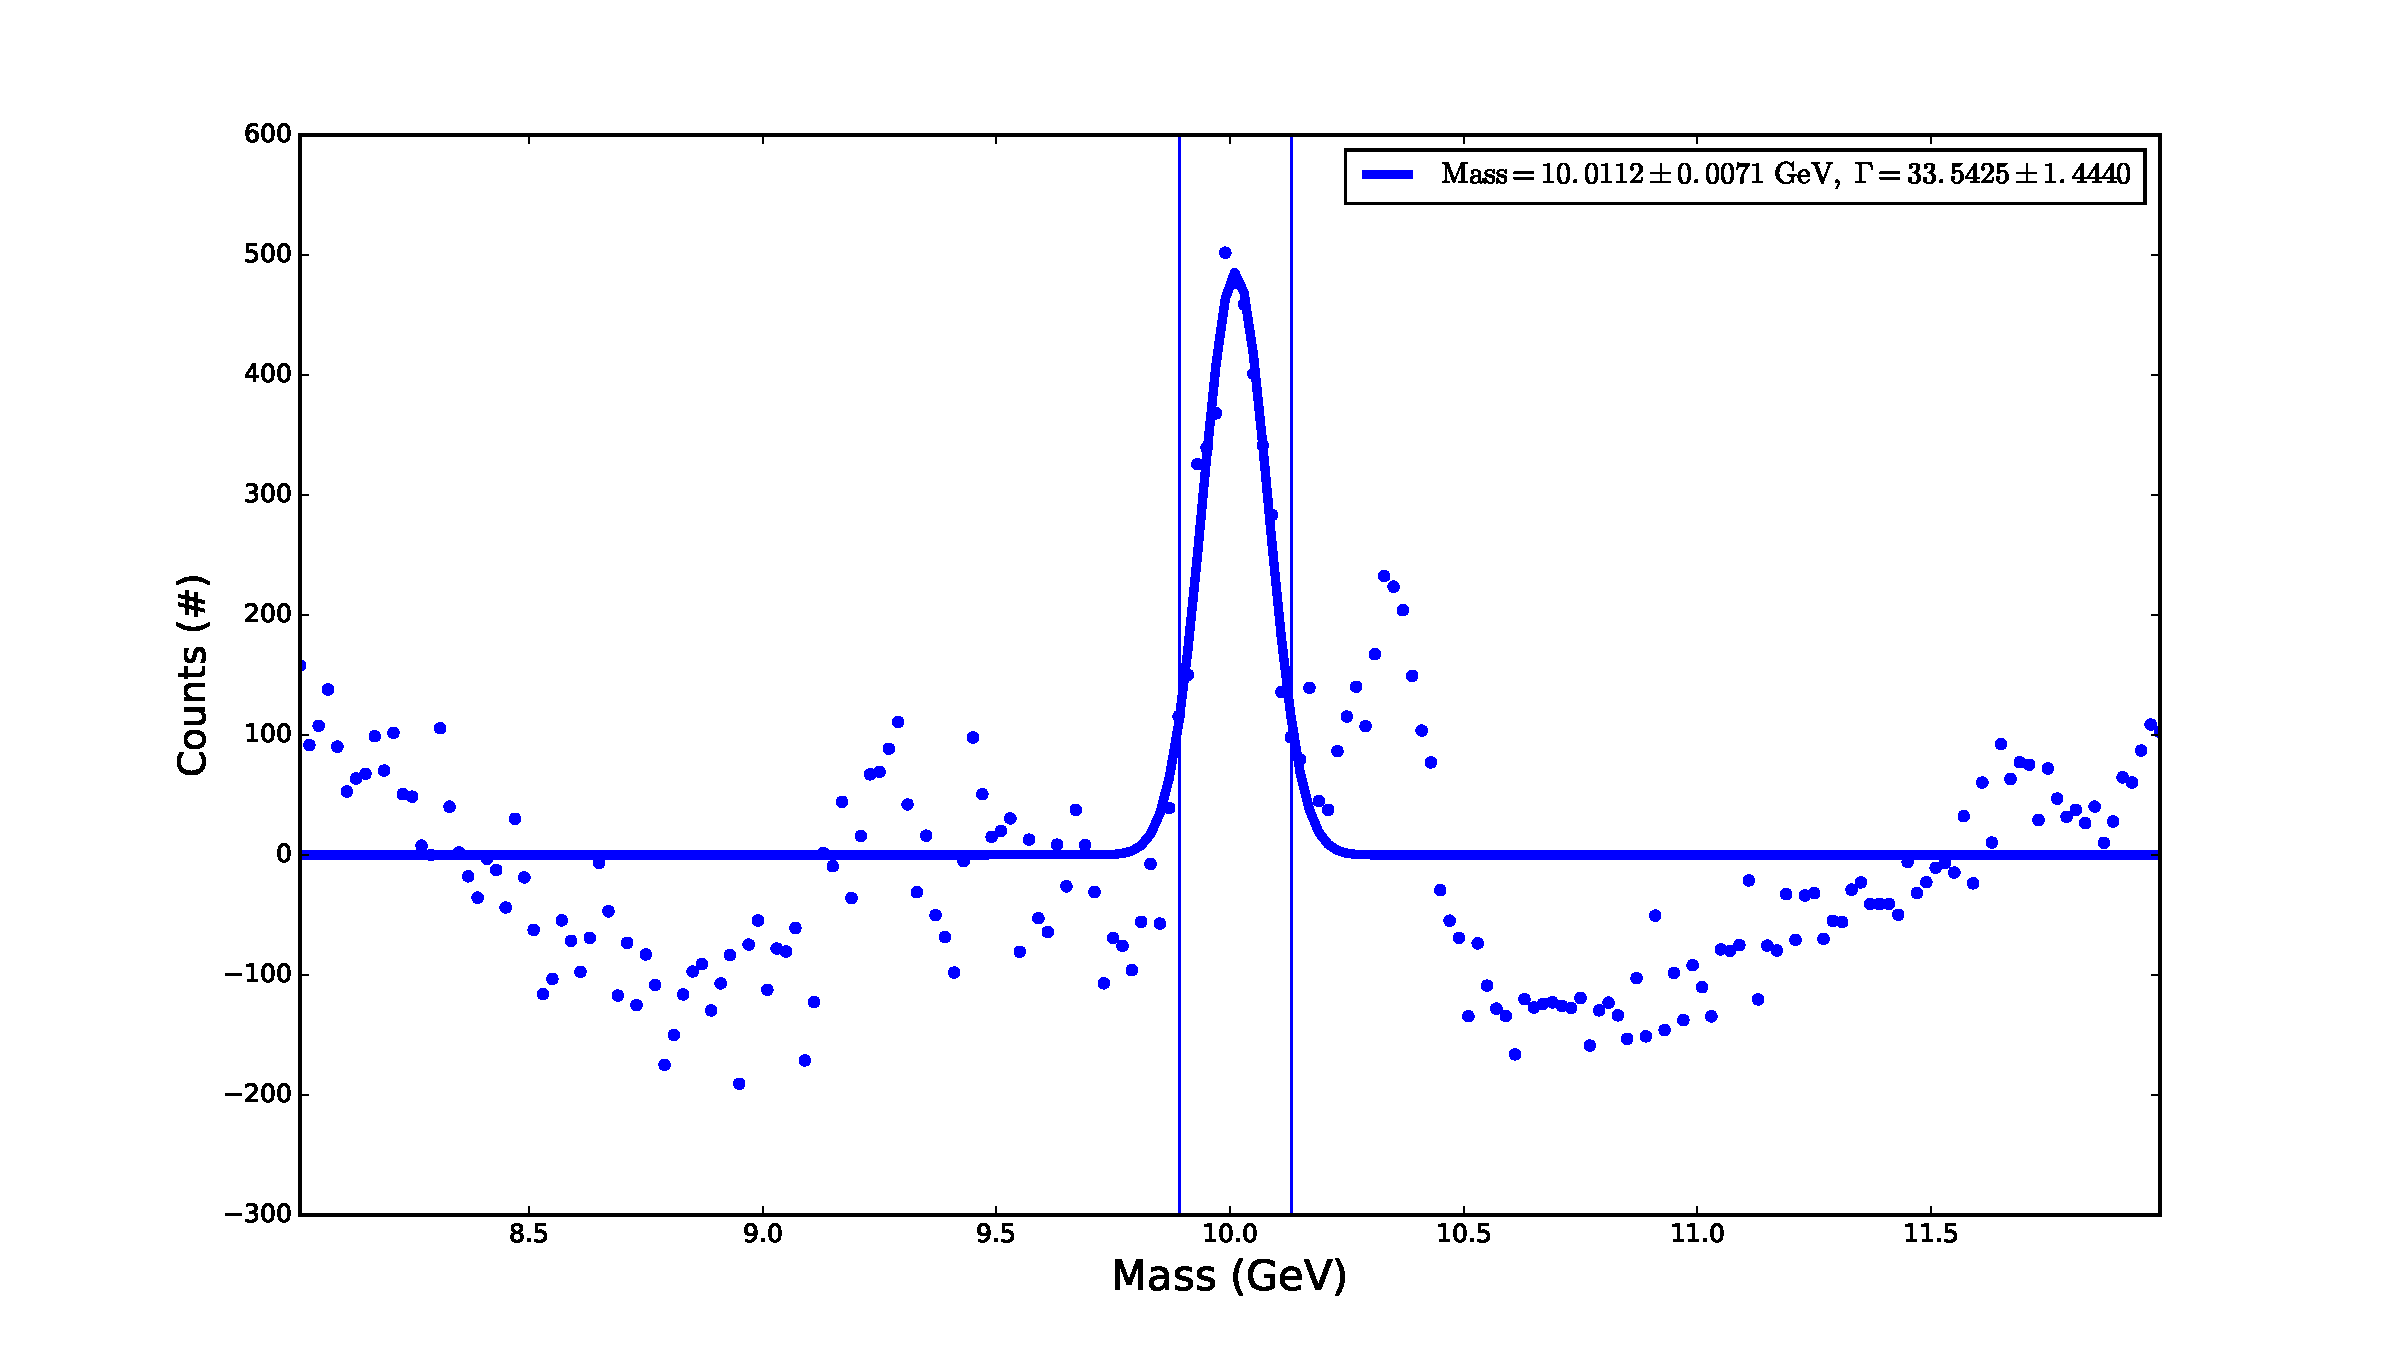
\includegraphics[width=\textwidth]{Upsilon/Up_peak.pdf} \\

\subsection*{Scatter Matrix}
Again to find interesting distributions I looked at the matrix of the scatter plots and looked at the  $\Upsilon$ Energy versus $\Upsilon$ Pz and $\Upsilon$ Energy versus $\Upsilon$ Pt \\
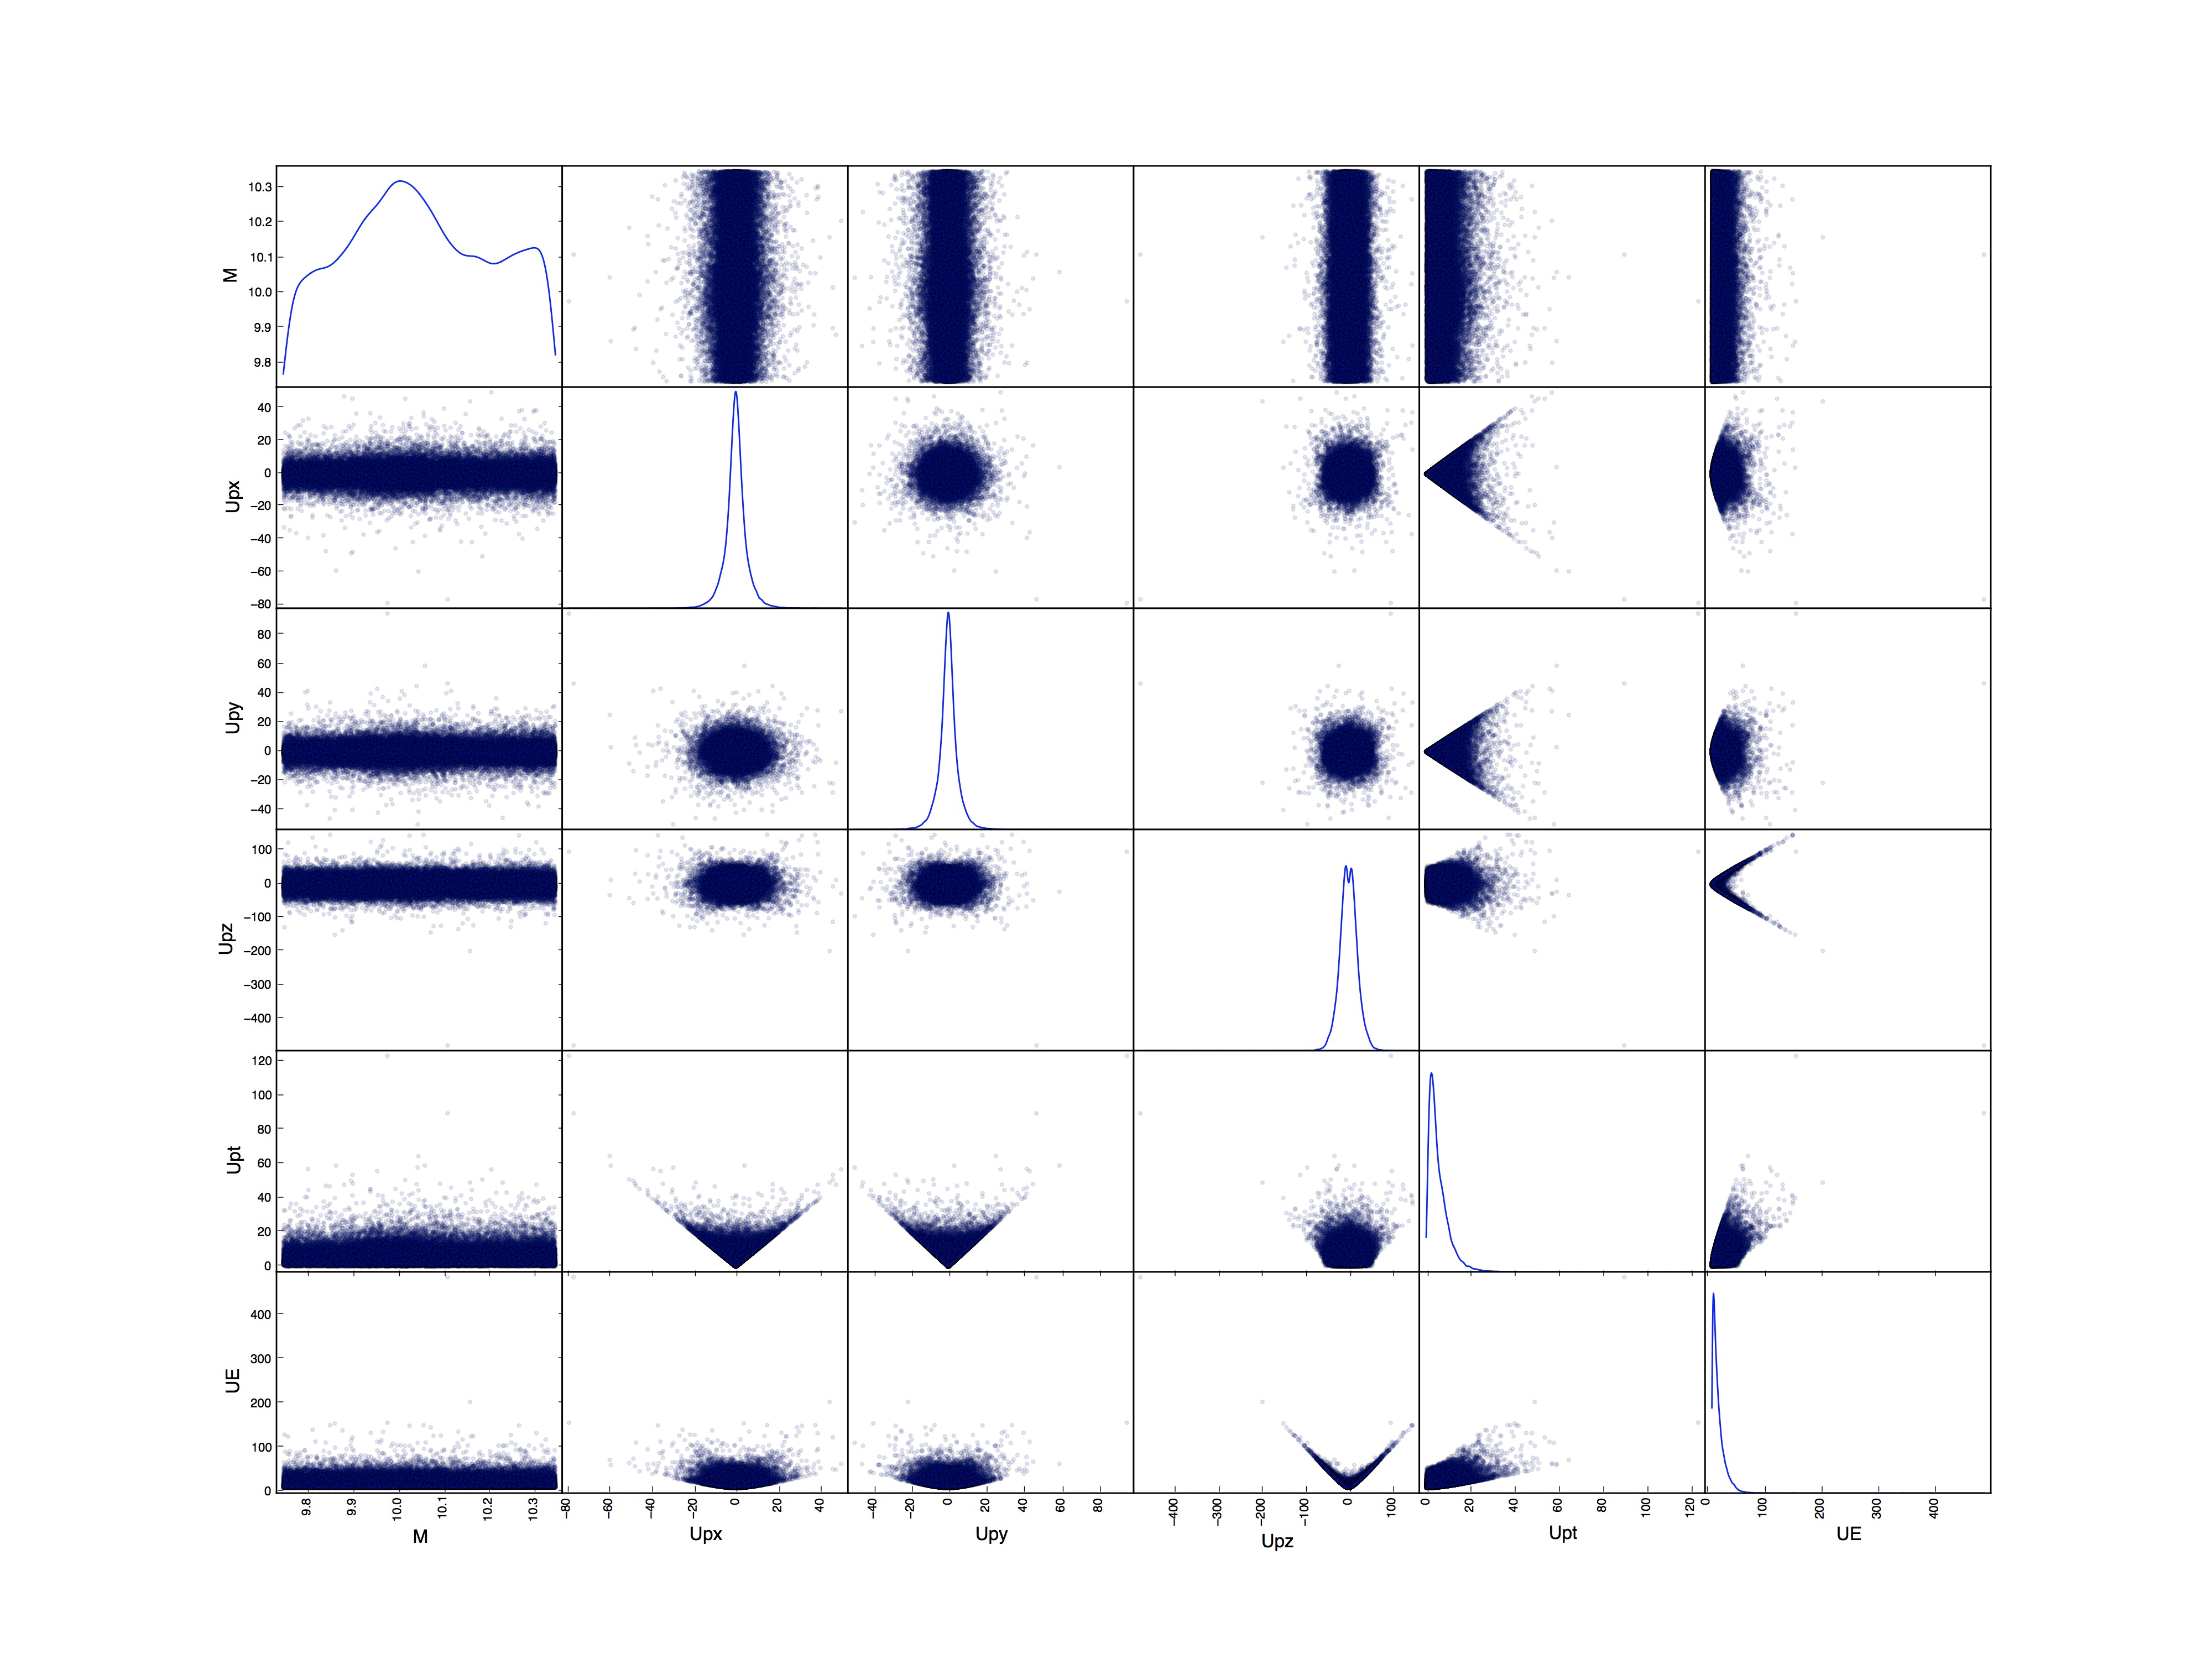
\includegraphics[width=0.9\textwidth]{Upsilon/scatter_matrix.jpg} \\

\subsection*{$\Upsilon$ Energy versus $\Upsilon$ Pz}
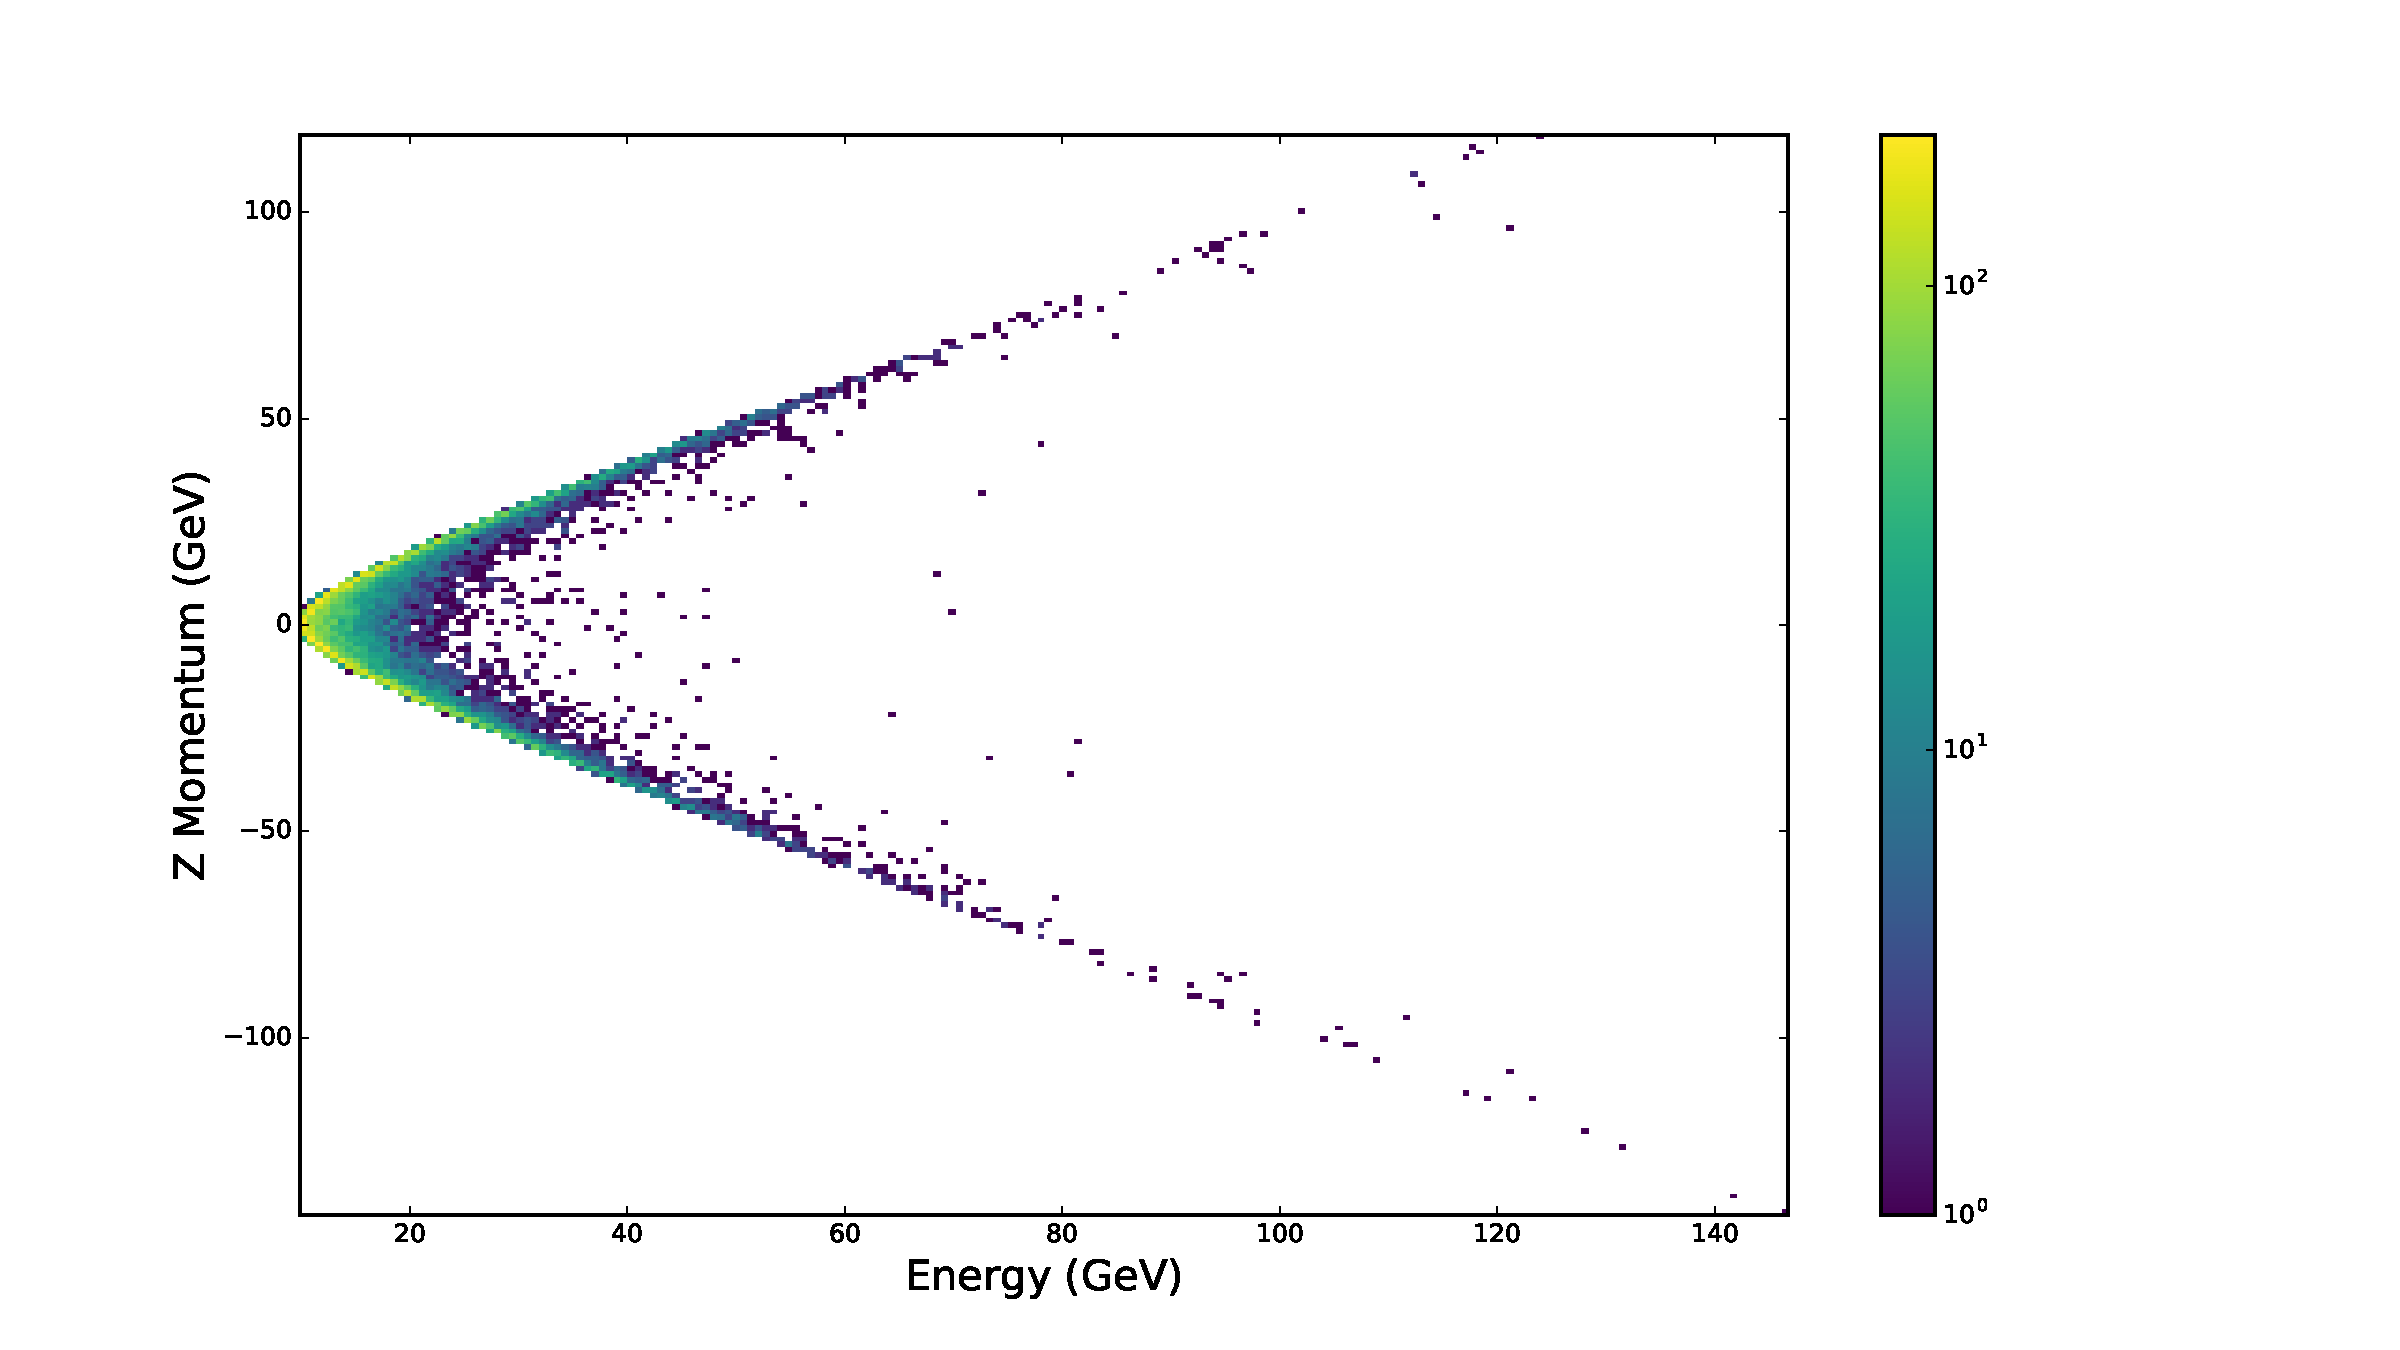
\includegraphics[width=\textwidth]{Upsilon/UE_Upz.pdf} \\

This distribution is slightly different then the $Z^0$ distribution. There is a larger range in the Z momentum distribution opposed to the large peak around 0 for the $Z^0$.  This can also be seen in the wide distribution seen on the Pz projection. \\

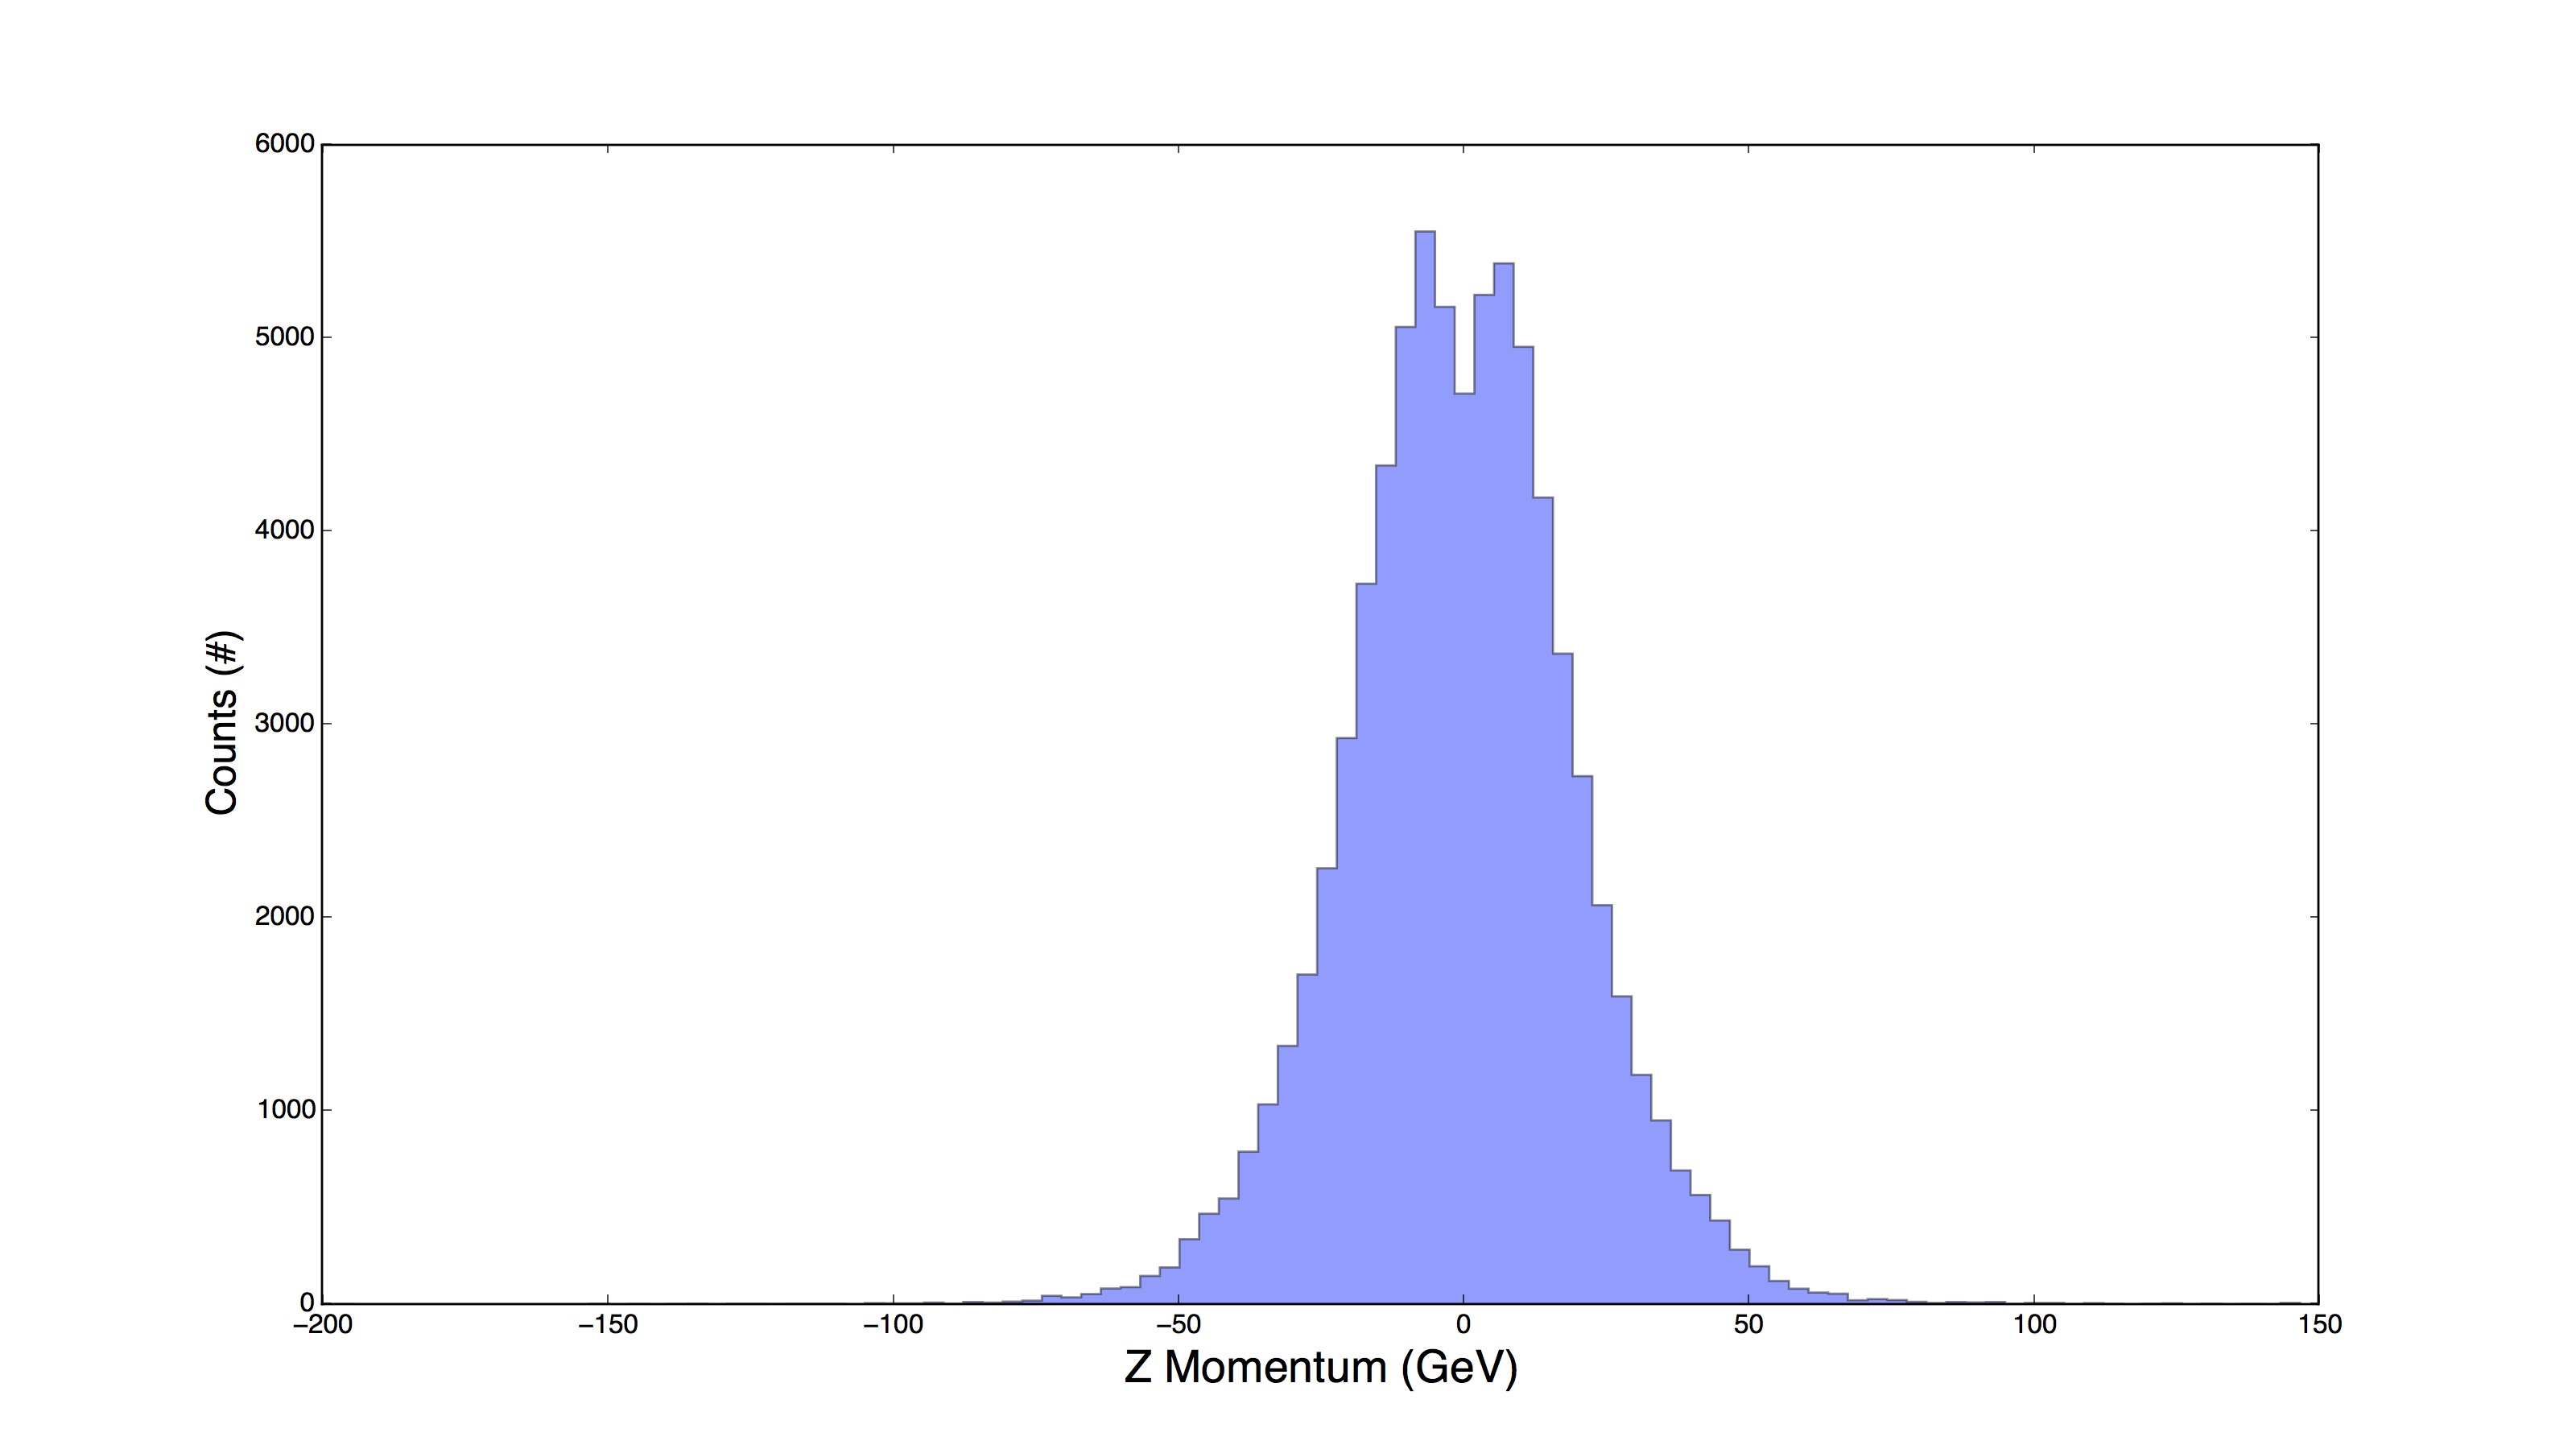
\includegraphics[width=\textwidth]{Upsilon/Upz.pdf} \\

However it is hard to tell whether this is due to something physical with the $\Upsilon$ production or if this is due to the background.  A better investigation into the backgrounds in this region could help to clear up the the particle identification process. \\ 

\subsection*{$\Upsilon$ Energy versus $\Upsilon$ Pt}
\includegraphics[width=\textwidth]{Upsilon/UE_Upt_log.pdf} \\

When first looking at the $\Upsilon$ Energy versus $\Upsilon$ Pt distribution one can see that there are a lot of events around the low energy, low momentum region.  In closer instigation in this region there seems to be two bands appearing.  The first band follows an arc with a slope close to one while the other is a wider and shallower band continuing in the low $Pt \approx 5\,GeV$ region.

\includegraphics[width=\textwidth]{Upsilon/UE_Upt_log_2.pdf} \\
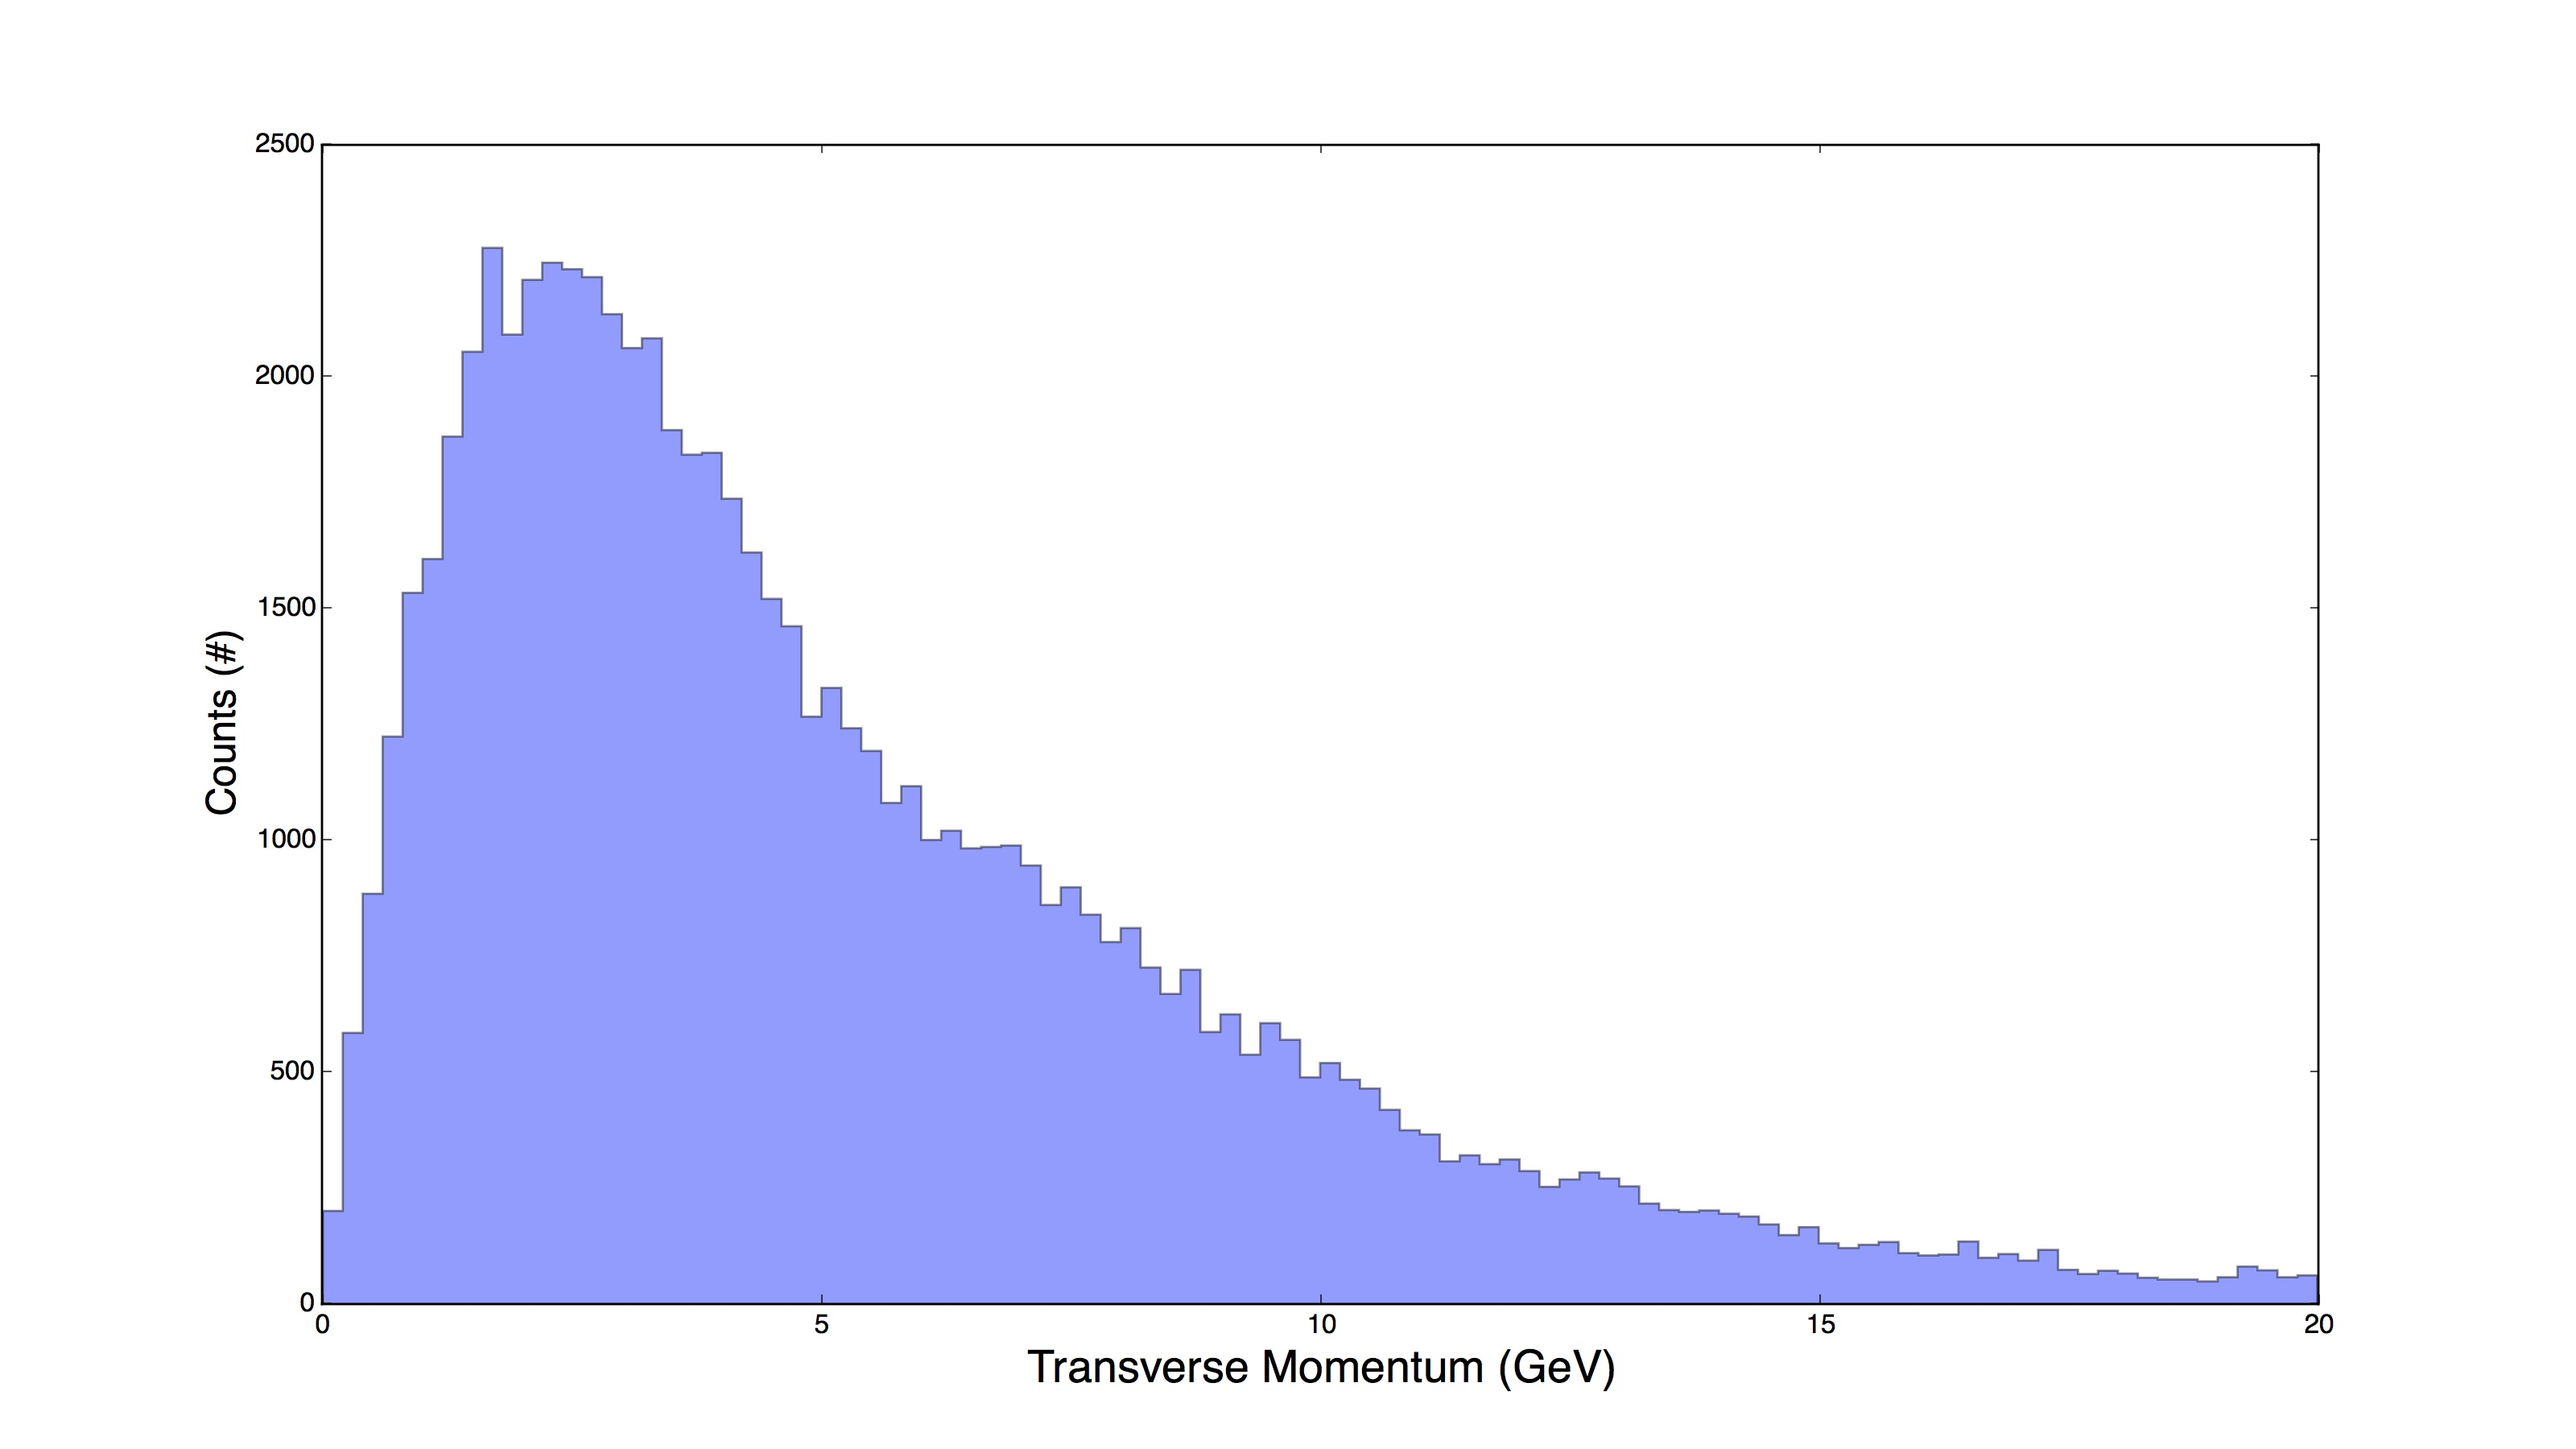
\includegraphics[width=\textwidth]{Upsilon/Upt.pdf} \\

With higher statistics this could become interesting to use this either for background subtraction or to look at the properties of high transverse momentum $\Upsilon$ versus low transverse momentum $\Upsilon$.

\begin{thebibliography}{}
\bibitem{OpenData}  CMS Open Data: (http://opendata.cern.ch/research/CMS).
\bibitem{GitHub} GitHub DiMuon Filter: (https://github.com/tpmccauley/dimuon-filter)
\end{thebibliography}

\end{document}

